
\chapter{Grothendieck \topos{}与空间的概念}

\philoquote{
	Le point de vue et le langage des faisceaux introduit par Leray nous a amené à regarder les ``espaces'' et ``variétés'' en tous genres dans une lumière nouvelle.
	Ils ne touchaient pas, pourtant, à la notion même d'espace, se contentant de nous faire appréhender plus finement, avec des yeux nouveaux, ces traditionnels ``espaces'',
	déjà familiers à tous.
	
	~\\
	
	%Or, il s'est avéré que cette notion d'espace est inadéquate pour rendre compte des ``invariants topologiques'' les plus essentiels qui expriment la ``forme'' des variétés algébriques ``abstraites'' (comme celles auxquelles s'appliquent les conjectures de Weil), voire celle des ``schémas'' généraux (généralisant les anciennes variétés).
	\quad[C]e qui compte vraiment dans un espace topologique, ce ne sont nullement ses ``points'' ou ses sous-ensembles de points, et les relations de proximité etc entre ceux-ci, mais que ce sont les faisceaux sur cet espace, et la catégorie qu'ils forment.
	}{Grothendieck, Récoltes et Semailles\footnotemark}
\footnotetext{这两段评注出自 Grothendieck 的自传 ``收获与播种''.
	
Leray 引入的层的观点和语言使我们以新的视角看待各种 ``空间'' 和 ``流形''. 然而, 它们并未触及空间的概念本身, 只是用新的眼光更加精细地理解那些传统的, 人们早已熟知的空间. % 然而, 事实证明, 这种空间的概念无法准确表达 ``抽象'' 代数簇 (如 Weil 猜想所使用的代数簇) 以及 (推广了传统代数簇的) 一般的 ``概形'' 最本质的 ``拓扑不变量''.

拓扑空间中真正重要的不是它的 ``点'' 或点集的子集, 以及点之间的邻近关系等等, 而是这个空间上的层, 以及它们构成的范畴.
}

\label{chapter-grothendieck-toposes}

\topos{}的概念最早由 Grothendieck 提出. 他将其命名为 topos\footnote{希腊文, ``位置''}, 意在表达这个概念是能够承载拓扑与几何直观的最广泛的概念.

拓扑空间 $X$ 上的层构成一个\topos{} $\operatorname{Sh}(X)$, 称为\emph{层\topos{}} (sheaf topos). 这个\topos{}很大程度上反映了空间 $X$ 的信息. Grothendieck 将层的概念由拓扑空间推广到了最一般的语境, 由此得到一种极为广泛的空间概念; 他将其命名为\emph{景} (site). 景上的层构成的范畴即是所谓 \emph{Grothendieck \topos{}}.

Grothendieck 的想法是, 一个\topos{}不一定来自普通的拓扑空间, 但由于它与 (拓扑空间上的) 层范畴极为相似的性质, 我们可以设想它是一个假想的空间上的层范畴, 即其中的对象是这个假想的空间之上的层. 这个想法也可视为代数--几何对偶的一例: 正如 Gelfand 考虑 Hausdorff 空间上的复值连续函数, Grothendieck 考虑空间上的 ``集合值连续函数''.

% 层\topos{}中的真值是 $X$ 的一个开集, 代表命题 ``在 $X$ 上的何处成立''. 从外部看, $X$ 上的层可视为沿着 $X$ ``一族连续变化的对象'', 而在层\topos{}的语言中, 一个层仿佛单个的对象.

% 这几句话放这里不合适. 该放哪里?

我们从层的一般概念讲起.

\section{预层}

%\subsection{范畴上的预层}

\begin{definition}{(小范畴上的预层)}
    设 $\mathsf C$ 是小范畴. 定义 $\mathsf C$ 上的\emph{预层} (presheaf) 是 $\mathsf C^{\op}$ 到 $\mathsf {Set}$ 的函子.
    记 $\mathsf C$ 上的预层范畴为 $\widehat {\mathsf C} := \mathsf {Fun}(\mathsf C^{\op},\mathsf {Set})$.
\end{definition}

预层 $F \colon \mathsf C^{\op} \to \mathsf {Set}$ 可视为一个假想的空间, 可用 $\mathsf C$ 的对象来\emph{探测} (probe). 我们对这个 ``空间'' 仅有的了解, 是 $\mathsf C$ 的对象 $c$ 到 $F$ 的假想态射 ``$c\to F$'' 的集合 $F(c)$, 以及态射 $d\to c$ 与假想态射 ``$c\to F$'' 的复合 $d\to c\to F$, 这给出集合的映射 $F(c) \to F(d)$.

由 $\mathsf C$ 的对象 $c$, 可得 $\mathsf C$ 上的预层 $\operatorname{Hom}_{\mathsf C}(-,c)$. 这事实上是 $\mathsf C$ 到 $\widehat {\mathsf C}$ 的嵌入.
\begin{definition}
    {(米田嵌入)}
    小范畴 $\mathsf C$ 的\emph{米田嵌入}是指函子
    $\yo\colon \mathsf C \to \widehat{\mathsf C}$,
    $c\mapsto \yo(c) = \operatorname{Hom}_{\mathsf C}(-,c)$. 米田嵌入的像 $\yo(c)$ 称为\emph{可表函子} (representable functor).
\end{definition}

\begin{remark}{}
    米田嵌入也可定义为函子 $\operatorname{Hom}\colon \mathsf C^{\op}\times\mathsf C \to \mathsf {Set}$ 对应的函子
    $\mathsf C \to \mathsf {Fun}(\mathsf C^{\op},\mathsf {Set})$. 这是因为 $\widehat {\mathsf {C}}$ 是 ``范畴的范畴'' 中的指数对象.
\end{remark}

对于预层 $F \in \widehat {\mathsf C}$, 前面提到的 $c$ 到 $F$ 的 ``假想态射'' 可赋予真实的含义, 它就是 $\yo(c)$ 到 $F$ 的态射 (自然变换). 这样一个自然变换由 $\operatorname{id}_c \in \yo(c)(c)$ 的像 ($F(c)$ 的元素) 唯一决定, 因此有如下的结论.
\begin{prop}{(米田引理)}
    对任意 $X \in \widehat {\mathsf C}$, 有自然同构
    $$
    \operatorname{Hom}_{\widehat {\mathsf C}}(\yo(c),F) \simeq F(c).
    $$
\end{prop}

\begin{remark}{}
    米田引理在逻辑上是平凡的; 它带给我们的\emph{观点}, 即 $\mathsf C$ 的对象 $c$ 可\emph{等同于}函子 $\yo(c)$, 比命题本身更重要. 后面我们将大量使用这种观点.

    关于米田引理的更多应用, 以及预层范畴的更多性质, 见附录 \ref{yoneda} 节.
\end{remark}

\subsection{常见的预层范畴}

\begin{example}
    {(集合)}
    记 $\mathsf {1}$ 为仅有一个对象和一个态射的范畴.
    $\mathsf {1}$ 上的预层范畴 $\widehat {\mathsf 1} = \mathsf {Set}^{\mathsf {1}^\op}$ 等同于集合范畴 $\mathsf {Set}$.
    它也可视为单点空间上的层范畴;
    它在\topos{}中扮演的角色等同于一个点在拓扑空间中扮演的角色.
\end{example}

\begin{example}
    [label={Simplicial-Sets}]
    {(单纯集)}
    令范畴 $\Delta$ 为有限全序集 $[0],[1],[2],\cdots$ 与保序映射构成的范畴, 其中 $[n] = \{0,1,\cdots,n\}$, 称映射 $f \colon [n] \to [m]$ 为保序映射是指当 $i\leq j$ 时 $f(i)\leq f(j)$.
    我们将 $[n]$ 想象为 $n$ 维单纯形.
    称范畴 $\Delta$ 为\emph{单纯范畴} (simplicial category).

    $\Delta$ 上的预层称为\emph{单纯集} (simplicial set), 也就是可用单纯形来探测的空间. 记单纯集范畴为
    $\mathsf {sSet}=\widehat {\Delta}=\mathsf {Fun}(\Delta^{\op},\mathsf {Set})$.
    
    对于单纯集 $X \colon 
    \Delta^{\op} \to \mathsf {Set}$,
    $X([n])$ 表示 $X$ 中 $n$ 维单形的集合,
    其中含有退化的单形.
    记米田嵌入 $\yo([n])$ 为 $\Delta^n$,
    米田引理告诉我们
    $$
    X([n]) \simeq \operatorname{Hom}_{\mathsf {sSet}}(\Delta^n,X),
    $$
    因此如上关于 $X([n])$ 的解释是准确的.
\end{example}

\begin{example}
    {(有向图)}
    有向图可用类似于单纯集 (例 \ref{Simplicial-Sets}) 的方式定义.
    考虑范畴
    $$
    \mathsf C=
    \Big\{\!
    \begin{tikzcd}[ampersand replacement=\&]
	{[0]} \& {[1]}
	\arrow["s", shift left, from=1-1, to=1-2]
	\arrow["t"', shift right, from=1-1, to=1-2]
    \end{tikzcd}
    \!\Big\},
    $$
    其中 $s,t\colon [0]\to [1]$
    分别将 $0\in [0]$ 映射到 $0\in [1]$ 和 $1\in [1]$.
    那么 $\mathsf C$ 上的预层 $X\colon \mathsf C^{\op}\to\mathsf {Set}$ 可视为有向图:
    $X([0])$ 是有向图的顶点集, $X([1])$ 是有向图的边集;
    映射 $X(s),X(t)\colon X([1])\to X([0])$ 将有向图的边对应到其起点与终点.
\end{example}

\begin{example}
    [label={G-set-presheaf-category}]
    {($G$-集)}
    设 $G$ 是群. 定义范畴 $\mathsf BG$ 为仅有一个对象的范畴,
    这个对象到自身的态射集为 $G$.

    $\mathsf BG$ 上的预层是函子 $(\mathsf B G)^{\op} \simeq \mathsf B(G^{\op}) \to \mathsf {Set}$, 等同于具有 $G^{\op}$-左作用即 $G$-右作用的集合, 也称为 $G$-集或 $G$ 的表示. 记 $G$-集的范畴为 $G\mathsf {Set}$.
\end{example}

%\subsection{拓扑空间上的预层}

范畴上预层的概念来自拓扑空间上的预层.
设 $X$ 为拓扑空间, 记 $\operatorname{Open}(X)$ 为 $X$ 的开集在包含关系下构成的范畴.

\begin{definition}
    {(拓扑空间上的预层)}
    拓扑空间 $X$ 上的\emph{预层}是 $\operatorname{Open}(X)$ 上的预层, 也即函子 $\operatorname{Open}(X)^{\op} \to \mathsf {Set}$.
    记 $X$ 上的预层范畴为 $\operatorname{Presh}(X)$.
\end{definition}

\begin{remark}
    {}
    需要注意的一点是, 拓扑空间 $X$ 到范畴 $\operatorname{Open}(X)$ 的对应是反变的, 也即对连续映射 $f\colon X \to Y$, 我们有反方向的函子 $f^{-1}\colon \operatorname{Open}(Y) \to \operatorname{Open}(X)$, 将开子集 $U\subset Y$ 对应到 $f^{-1}(U)\subset X$.
\end{remark}

下面我们说明小范畴 $\mathsf C$ 上的预层范畴 $\widehat {\mathsf C}$ 是一个\topos{}.

\begin{prop}
	[label={presheaf-category-complete}]
	{(预层范畴完备且余完备)}
    $\widehat {\mathsf C}$ 是\emph{完备} (complete) 且\emph{余完备} (cocomplete) 的, 也即具有一切 (小) 极限与余极限.
\end{prop}

\begin{proof}
    预层的极限可 ``逐点'' 计算: 设 $F \colon I \to \widehat {\mathsf C}, i \mapsto F_i$ 是任意图表, 那么其极限为
    $$
    \big(\lim_I F_i\big)(c) = \lim_I F_i(c),
    $$
    余极限类似.
\end{proof}

特别地, 预层范畴 $\widehat {\mathsf C}$ 的终对象 (空图的极限) 是将所有对象 $c$ 对应到 $\mathsf {Set}$ 的终对象 $1$ 的预层, 而始对象 (空图的余极限) 将所有对象对应到 $\mathsf {Set}$ 的始对象 $\varnothing$.
预层的积与和即是逐点的积与和.

\begin{prop}
	[label={presheaf-category-exponential}]
	{}
    $\widehat{\mathsf C}$ 是积闭范畴.
\end{prop}

\begin{proof}
    对 $X,Y \in \widehat {\mathsf C}$,
    我们不能以 $Y^X(c) = Y(c)^{X(c)}$ 来定义指数对象 $Y^X$, 因为这个构造没有函子性.
    一种可行的思路如下. 假设指数对象 $Y^X$ 存在, 即有 (关于 $Z$ 的) 自然同构
    $$
    \operatorname{Hom}_{\widehat{\mathsf C}}(Z,Y^X) \simeq \operatorname{Hom}_{\widehat{\mathsf C}}(Z\times X,Y).
    $$
    代入 $Z=\yo(c)$, 由米田引理便得到 (关于 $c$ 的) 自然同构
    $$
    Y^X(c) = \operatorname{Hom}_{\widehat{\mathsf C}}(\yo(c)\times X,Y),
    $$
    这已经确定了函子 $Y^X$.
    下面验证这个函子确实满足指数对象的条件.

    首先给出取值映射 $\operatorname{ev} \colon Y^X \times X \to Y$,
    也即自然的映射
    $$
    \operatorname{Hom}_{\widehat C}(\yo(c)\times X,Y)\times X(c)\to Y(c).
    $$
    对 $\theta \in \operatorname{Hom}_{\widehat C}(\yo(c)\times X,Y)$,
    考虑 $\theta_c \colon \yo(c)(c)\times X(c) \to Y(c)$,
    代入 $\operatorname{id}_c$ 便得到映射 $X(c)\to Y(c)$.
    
\end{proof}

\subsection{筛与预层范畴中的子对象}

本节的目标是如下命题.

\begin{prop}
    [label={presheaf-category-subobject-classifier}]
    {}
    $\widehat{\mathsf C}$ 具有子对象分类子.
\end{prop}

    首先我们描述 $\widehat{\mathsf C}$ 中的子对象.

\begin{propdef}
    [label={subfunctor-description}]
    {(子函子)}
    $\widehat{\mathsf C}$ 中的态射 $Y \to X$ 是单射, 当且仅当对每个对象 $c$, 映射 $Y(c) \to X(c)$ 都是子集,
    且对每个态射 $c\to d$, 映射 $Y(d) \to Y(c)$ 都是 $X(d) \to X(c)$ 的限制; 此时也称 $Y \to X$ 为\emph{子函子} (subfunctor).
\end{propdef}

\begin{proof}
	由单射的拉回刻画 (命题 \ref{mono-epi-pullback-pushout}) 以及 $\widehat {\mathsf C}$ 中极限的逐点计算 (命题 \ref{presheaf-category-complete}) 即证.
\end{proof}

\emph{筛}的概念可帮助描述预层范畴的子对象分类子.

\begin{definition}
	[label={sieve}]
    {(筛)}
    范畴 $\mathsf C$ 的对象 $c$ 上的一个\emph{筛} (英 sieve, 法 crible) 是指 $\mathsf C$ 中一族指向 $c$ 的箭头 \makebox{$S= \{f \colon d \to c\}$}, 构成 $\mathsf C$ 的\emph{右理想}; 也即对任意 $f\in S$ 与 $\mathsf C$ 中任意箭头 $g$, 只要 $fg$ 可定义, 就有 $fg \in S$.

    对于两个筛 $R,S$, 若 $R\subset S$, 则称 $R$ 比 $S$ 更细, 或 $R$ 是 $S$ 的一个\emph{细化} (refinement).

    设 $R$ 是一族指向 $c$ 的箭头. 定义 $R$ \emph{生成}的筛为  $\{e\to d\to c\mid (d\to c)\in R \}$, 也即包含 $R$ 中所有箭头的最细的筛.
\end{definition}

\begin{remark}
    {(筛的直观)}
    筛是一种能把大的东西挡住, 让小的东西通过的工具. 想象 $S$ 的元素为可以 ``通过'' $S$ 的箭头.
    若 $d \overset{f}{\longrightarrow} c$ 可以 ``通过'' $S$, 那么 $e \overset{g}{\longrightarrow} d \overset{f}{\longrightarrow} c$ 比 $d \overset{f}{\longrightarrow} c$ ``小'', 从而它也可以 ``通过'' $S$.

    \begin{center}
        

\tikzset{every picture/.style={line width=0.75pt}} %set default line width to 0.75pt        

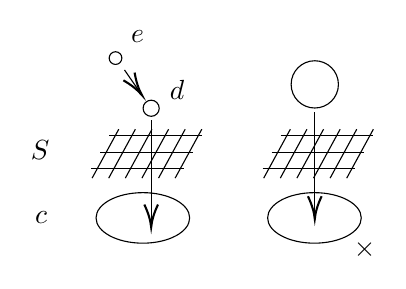
\begin{tikzpicture}[x=0.75pt,y=0.75pt,yscale=-1,xscale=1]
%uncomment if require: \path (0,300); %set diagram left start at 0, and has height of 300

%Shape: Ellipse [id:dp10401378338786049] 
\draw   (74,113.39) .. controls (74,106.67) and (84.1,101.22) .. (96.56,101.22) .. controls (109.01,101.22) and (119.11,106.67) .. (119.11,113.39) .. controls (119.11,120.11) and (109.01,125.56) .. (96.56,125.56) .. controls (84.1,125.56) and (74,120.11) .. (74,113.39) -- cycle ;
%Shape: Grid [id:dp09583060841478219] 
\draw  [draw opacity=0] (81.95,70.67) -- (126.56,70.67) -- (113.72,94.22) -- (69.11,94.22) -- cycle ; \draw   (84.95,70.67) -- (72.11,94.22)(92.95,70.67) -- (80.11,94.22)(100.95,70.67) -- (88.11,94.22)(108.95,70.67) -- (96.11,94.22)(116.95,70.67) -- (104.11,94.22)(124.95,70.67) -- (112.11,94.22) ; \draw   (80.31,73.67) -- (124.92,73.67)(75.95,81.67) -- (120.56,81.67)(71.59,89.67) -- (116.2,89.67) ; \draw    ;
%Shape: Circle [id:dp31189924819685966] 
\draw   (80.33,36.39) .. controls (80.33,34.7) and (81.7,33.33) .. (83.39,33.33) .. controls (85.08,33.33) and (86.44,34.7) .. (86.44,36.39) .. controls (86.44,38.08) and (85.08,39.44) .. (83.39,39.44) .. controls (81.7,39.44) and (80.33,38.08) .. (80.33,36.39) -- cycle ;
%Straight Lines [id:da12935033787340267] 
\draw    (87.72,42.11) -- (94.97,52.58) ;
\draw [shift={(96.11,54.22)}, rotate = 235.29] [color={rgb, 255:red, 0; green, 0; blue, 0 }  ][line width=0.75]    (10.93,-3.29) .. controls (6.95,-1.4) and (3.31,-0.3) .. (0,0) .. controls (3.31,0.3) and (6.95,1.4) .. (10.93,3.29)   ;
%Shape: Circle [id:dp7222065551952845] 
\draw   (96.67,60.56) .. controls (96.67,58.41) and (98.41,56.67) .. (100.56,56.67) .. controls (102.7,56.67) and (104.44,58.41) .. (104.44,60.56) .. controls (104.44,62.7) and (102.7,64.44) .. (100.56,64.44) .. controls (98.41,64.44) and (96.67,62.7) .. (96.67,60.56) -- cycle ;
%Straight Lines [id:da7276461675375434] 
\draw    (100.56,66.44) -- (100.56,115.89) ;
\draw [shift={(100.56,117.89)}, rotate = 270] [color={rgb, 255:red, 0; green, 0; blue, 0 }  ][line width=0.75]    (10.93,-3.29) .. controls (6.95,-1.4) and (3.31,-0.3) .. (0,0) .. controls (3.31,0.3) and (6.95,1.4) .. (10.93,3.29)   ;
%Shape: Ellipse [id:dp12697611260252684] 
\draw   (156.67,113.39) .. controls (156.67,106.67) and (166.77,101.22) .. (179.22,101.22) .. controls (191.68,101.22) and (201.78,106.67) .. (201.78,113.39) .. controls (201.78,120.11) and (191.68,125.56) .. (179.22,125.56) .. controls (166.77,125.56) and (156.67,120.11) .. (156.67,113.39) -- cycle ;
%Shape: Grid [id:dp9936460967678797] 
\draw  [draw opacity=0] (164.61,70.67) -- (209.22,70.67) -- (196.39,94.22) -- (151.78,94.22) -- cycle ; \draw   (167.61,70.67) -- (154.78,94.22)(175.61,70.67) -- (162.78,94.22)(183.61,70.67) -- (170.78,94.22)(191.61,70.67) -- (178.78,94.22)(199.61,70.67) -- (186.78,94.22)(207.61,70.67) -- (194.78,94.22) ; \draw   (162.98,73.67) -- (207.59,73.67)(158.62,81.67) -- (203.23,81.67)(154.26,89.67) -- (198.87,89.67) ; \draw    ;
%Shape: Circle [id:dp838751100400853] 
\draw   (168,49.06) .. controls (168,42.77) and (173.1,37.67) .. (179.39,37.67) .. controls (185.68,37.67) and (190.78,42.77) .. (190.78,49.06) .. controls (190.78,55.35) and (185.68,60.44) .. (179.39,60.44) .. controls (173.1,60.44) and (168,55.35) .. (168,49.06) -- cycle ;
%Straight Lines [id:da5932706956135338] 
\draw    (179.39,62.44) -- (179.39,111.89) ;
\draw [shift={(179.39,113.89)}, rotate = 270] [color={rgb, 255:red, 0; green, 0; blue, 0 }  ][line width=0.75]    (10.93,-3.29) .. controls (6.95,-1.4) and (3.31,-0.3) .. (0,0) .. controls (3.31,0.3) and (6.95,1.4) .. (10.93,3.29)   ;

% Text Node
\draw (43.33,109) node [anchor=north west][inner sep=0.75pt]   [align=left] {$\displaystyle c$};
% Text Node
\draw (41.33,75) node [anchor=north west][inner sep=0.75pt]   [align=left] {$\displaystyle S$};
% Text Node
\draw (113,123.67) node [anchor=north west][inner sep=0.75pt]   [align=left] {$\displaystyle \checkmark$};
% Text Node
\draw (197,123) node [anchor=north west][inner sep=0.75pt]   [align=left] {$\displaystyle \times $};
% Text Node
\draw (108.33,46) node [anchor=north west][inner sep=0.75pt]   [align=left] {$\displaystyle d$};
% Text Node
\draw (89.67,22) node [anchor=north west][inner sep=0.75pt]   [align=left] {$\displaystyle e$};


\end{tikzpicture}
    \end{center}

    % 这里, 我们认为指向 $c$ 的态射越复合就越小. 回忆环是一个对象的 $\mathsf {Ab}$-充实范畴, 那么其中的筛正是环的右理想; 筛的大小观念类似于 $p$-进度量下的整数越乘越小.

    一个筛越细, 能 ``通过'' 它的东西就越少, 这解释了\emph{细化}的含义.
\end{remark}

\begin{example}
	[label={sieve-from-cover}]
	{(覆盖产生筛)}
	设 $X$ 为拓扑空间, $\{U_i\}$ 是其中开集 $V$ 的一个开覆盖. 那么
	$$
	\big\{W\subset V \mid \exists i, W \subset U_i\big\}
	$$
	构成 $\operatorname{Open}(X)$ 中 $V$ 上的一个筛. 直观上每个 $U_i$ 是筛上的一个 ``洞'', 比它小的对象能 ``通过'' 这个筛.
\end{example}

\begin{prop}
	[label={sieve-and-subfunctor}]
    {(筛与子函子)}
    范畴 $\mathsf C$ 的对象 $c$ 上的筛自然地一一对应于 $\yo(c)$ 的子函子.
\end{prop}

\begin{proof}
    设 $S$ 是 $c$ 上的筛, 那么
    $$
    X(d) = \{f\colon d\to c \mid f\in S\} \subset \operatorname{Hom}_{\mathsf C}(d,c) = \yo(c)(d)
    $$
    构成 $\yo(c)$ 的子函子.
    设 $X \to \yo(c)$ 为子函子, 那么
    $$
    S=\big\{
        f \colon d\to c \mid f\in X(d)
    \big\}
    $$
    是 $c$ 上的筛. 很明显, 这两个对应是互逆的.
\end{proof}

\begin{remark}
    {}
    若将 $\widehat {\mathsf C}$ 的对象称作 $\mathsf C$ 的 ``广义对象'', 那么 $\yo(c)$ 的子函子可称作 $c$ 的 ``广义子对象''.

    $\mathsf C$ 的 ``广义对象'' $X$ 的子对象, 根据命题 \ref{subfunctor-description} 的描述, 也可视为 $X$ 上的 ``筛''.
\end{remark}

\begin{example}
	[label={sieve-from-cover-subfunctor}]
	{(覆盖产生的筛对应的子函子)}
	继续例 \ref{sieve-from-cover}, 设 $S$ 为覆盖 $\{U_i\}$ 生成的筛对应的 $\yo(V)$ 的子函子, 那么下图是余等化子.
	\begin{equation}
		\label{sieve-coeq}
		\begin{tikzcd}[ampersand replacement=\&]
			{\coprod_{i,j}\yo(U_i\cap U_j)} \& {\coprod_i \yo(U_i)} \& S
			\arrow[shift right, from=1-1, to=1-2]
			\arrow[shift left, from=1-1, to=1-2]
			\arrow[from=1-2, to=1-3]
		\end{tikzcd}
	\end{equation}
	这是因为, 由 $S$ 的定义, 对 $W\in\operatorname{Open}(X)$, 若存在 $i$, $W\subset U_i$ 则 $S(W)$ 是单元集; 否则 $S(W)$ 是空集. 由此可知下图是集合范畴中的余等化子.
	\[\begin{tikzcd}[ampersand replacement=\&, column sep=small]
		{\coprod_{i,j}\operatorname{Hom}_{\operatorname{Open}(X)}(W,U_i\cap U_j)} \& {\coprod_i \operatorname{Hom}_{\operatorname{Open}(X)}(W,U_i)} \& {S(W)}
		\arrow[shift right, from=1-1, to=1-2]
		\arrow[shift left, from=1-1, to=1-2]
		\arrow[from=1-2, to=1-3]
	\end{tikzcd}\]
	而预层的余极限是 ``逐点'' 的, 于是得 (\ref{sieve-coeq}).
	
	对 $X$ 上的任意预层 $F$, 以 $\operatorname{Hom}_{\operatorname{Presh}(X)}(-,F)$ 作用于 (\ref{sieve-coeq}), 可知下图是集合范畴中的等化子.
	\begin{equation}
		\begin{tikzcd}[ampersand replacement=\&]
			{\operatorname{Hom}_{\operatorname{Presh}(X)}(S,G)} \& {\prod_i G(U_i)} \& {\prod_{i,j}G(U_i\cap U_j)}
			\arrow[shift left, from=1-2, to=1-3]
			\arrow[shift right, from=1-2, to=1-3]
			\arrow[from=1-1, to=1-2]
		\end{tikzcd}
		\label{sieve-subfunctor-equalizer}
	\end{equation}
	因此态射集合 $\operatorname{Hom}_{\operatorname{Presh}(X)}(S,F)$ 表达了预层 $F$ 关于覆盖 $\{U_i\}$ 的下降资料 (descent data), 由覆盖 $\{U_i\}$ ``下降'' 到 $V$. 若 $F$ 为层, 就应该有 $$\operatorname{Hom}_{\operatorname{Presh}(X)}(S,F) \simeq F(V) \simeq \operatorname{Hom}_{\operatorname{Presh}(X)}(\yo(V),F).$$
\end{example}

\begin{example}
	[label={maximal-sieve}]
    {(极大筛)}
    所有指向 $c$ 的箭头的集合称为\emph{极大筛}, 也即最粗的筛.
    它对应 $\yo(c)$ 的子对象 $\yo(c)$ 自身 ($\yo(c)$ 到自身的恒等态射).
    注意, $c$ 上的一个筛是极大筛当且仅当它包含 $\operatorname{id}_c$.
\end{example}

现在我们给出命题 \ref{presheaf-category-subobject-classifier} 的证明.

\begin{proof}
    

    假设 $\widehat{\mathsf C}$ 中存在子对象分类子 $\Omega$, 那么由米田引理, 有自然同构
    $$
    \Omega(c) \simeq \operatorname{Hom}_{\widehat {\mathsf C}}(\yo(c),\Omega)
    \simeq \operatorname{Sub}_{\widehat {\mathsf C}}(\yo(c)),
    $$
    即
    $$
    \Omega(c) = \{\text{$c$ 上的筛}\},
    $$
    这便确定了函子 $\Omega$.
    下面验证这个函子确实满足 $\widehat{\mathsf C}$ 中子对象分类子的条件.

    定义态射 $\top\colon 1 \to \Omega,$
    对每个对象 $c$ 选出 $\Omega(c)= \operatorname{Sub}_{\widehat {\mathsf C}}(\yo(c))$
    中的子对象 $\yo(c)$ 自身, 也即 $c$ 上的极大筛.
    
    下面验证子对象分类子的条件. 设 $Y\to X$ 是 $\widehat{\mathsf C}$ 中的子对象.
    定义态射 $\chi \colon X \to \Omega$, 将 $x\in X(c)$ 对应到 $c$ 上的筛
    $$
    \chi(x) = \big\{f \colon d \to c \mid X(f)(x) \in Y(d)\big\}.
    $$
    注意 $\chi(x)$ 是极大筛当且仅当 $\operatorname{id}_c \in \chi(x)$, 也即 $x \in Y(c)$,
    所以子对象 $Y\to X$ 是如下的拉回.
    % https://q.uiver.app/#q=WzAsNCxbMCwxLCJYIl0sWzEsMSwiXFxPbWVnYSJdLFsxLDAsIjEiXSxbMCwwLCJZIl0sWzMsMF0sWzAsMSwiXFxjaGkiLDJdLFsyLDEsIlxcdG9wIl0sWzMsMl1d
    \[\begin{tikzcd}[ampersand replacement=\&]
    	Y \& 1 \\
    	X \& \Omega
    	\arrow[from=1-1, to=2-1]
    	\arrow["\chi"', from=2-1, to=2-2]
    	\arrow["\top", from=1-2, to=2-2]
    	\arrow[from=1-1, to=1-2]
    \end{tikzcd}\]
\end{proof}

综合上述论证, 我们得到
\begin{prop}{}
    $\widehat {\mathsf C}$ 是一个\topos{}.
\end{prop}

\begin{example}
    {($G$-集)}
    例 \ref{G-set-presheaf-category} 介绍了 $G$-集范畴, 即 $\mathsf BG$ 上的预层范畴. 由于 $\mathsf BG$ 只有一个对象且态射均为自同构,
    其上仅有两个筛, 空集与极大筛.
    
    因此, $G$-集范畴的子对象分类子 $\Omega$ 是二元集合 $\{\top,\bot\}$, 其上带有 $G$ 的平凡作用.
    事实上, 一个 $G$-集 $X$ 的子对象 $Y$ 是其中 $G$-作用下封闭的子集. 其对应的特征函数 $X\to\{\top,\bot\}$ 就是子集 $Y$ 的特征函数.
\end{example}


\section{层与景}

拓扑空间上的\emph{层}是满足 ``粘合'' 条件的预层; 一个开集上的截面\footnote{预层 $F$ 在 $U$ 上的\emph{截面} (section) 就是指 $F(U)$ 的元素. 这个术语来自于几何.}可由这个开集的任何一个覆盖上一族相容的截面唯一决定.

\begin{definition}
    {(拓扑空间上的层)}
    拓扑空间 $X$ 上的\emph{层} (sheaf) 是满足如下条件的预层 $F$:
    对任意开集 $U\subset X$, 任意覆盖 $U = \bigcup_i U_i$,
    以及任意一组相容的元素 \makebox{$(s_i \in F(U_i))_{i\in I}$},
    存在唯一的 $s\in F(U)$
    满足 $s|_{U_i} = s_i\,\forall i\in I$.
    其中相容是指
    \begin{equation}
        s_i|_{U_i\cap U_j} = s_j|_{U_i\cap U_j}\,(\forall i,j \in I),
        \label{sheaf-condition}
    \end{equation}
\end{definition}

Grothendieck 意识到, 层的概念所需的关键信息是一个对象 $U$ 何时被一族进入 $U$ 的态射 (甚至不一定是 $U$ 的子对象) 所\emph{覆盖}.

\subsection{从覆盖到 Grothendieck 拓扑}

本小节有许多的定义, 在读者看来这些定义可能有些冗余. 这或许是历史的遗留, 但每个定义有各自的长处.

\begin{definition}{(覆盖结构)}
    设范畴 $\mathsf C$ 具有拉回.
    $\mathsf C$ 上的一个\emph{覆盖结构} (coverage) $T$ 是如下结构: 对每个对象 $c$ 指定一个集合 $T(c)$, 其元素为态射族 $\{f_i \colon c_i \to c\}_{i\in I}$, 称为 $c$ 的 $T$-\emph{覆盖族} (covering family), 满足
    \begin{itemize}
    	\item (拉回下的稳定性) 若 $\{f_i \colon c_i \to c\}_{i\in I}\in T(c)$, $g \colon d \to c$,
    	则 $\{g^*(f_i) \colon d_i \to d\}_{i\in I}\in T(d)$.
    \end{itemize}
        
    %带有覆盖结构的范畴 $(\mathsf C,T)$ 称为\emph{景} (site).
    对于两个覆盖结构 $T,T'$, 若 $T$-覆盖族都是 $T'$-覆盖族, 则称 $T'$ 较\emph{细} (fine).
\end{definition}

对于拓扑空间的开集范畴, 拉回下的稳定性相当于若一族开集覆盖了 $U$, 那么它们也覆盖了 $U$ 的任何子集.

\begin{remark}
    {}
    当 $\mathsf C$ 不存在拉回时, ``拉回下的稳定性'' 可改为: 若 $\{f_i \colon c_i \to c\}_{i\in I}\in T(c)$, $g \colon d \to c$,
    则存在 $\{h_j \colon d_j \to d\}_{j\in J}\in T(d)$,
    使得每个 $gh_j$ 都穿过某个 $f_i$.
\end{remark}

%\begin{remark}{}
%    上面定义的覆盖结构有时也称为范畴上的 \emph{Grothendieck 拓扑}, 但这个词的含义有时要窄一些.
%\end{remark}

\begin{definition}
	[label={sheaf-condition}]
	{(关于态射族的层条件)}
	
	设 $F$ 是范畴 $\mathsf C$ 上的预层. 设 $M = \{f_i\colon c_i\to c\}_{i\in I}$ 是 $\mathsf C$ 中的一族态射. 称 $F$ 满足关于 $M$ 的\emph{层条件}, 是指对任意一组相容的元素 $(s_i\in F(c_i))_{i\in I}$,
	存在唯一的 $s\in F(c)$ 满足 $F(f_i)(s)=s_i\,\forall i\in I$.
	其中, 一组元素 $(s_i\in F(c_i))_{i\in I}$ \emph{相容}是指对任意态射 $f\colon d \to c_i$, $g\colon d \to c_j$, 有 $F(f)(s_i) = F(g)(s_j) \in F(d)$.
	
	在 $\mathsf C$ 具有拉回的条件下, 层条件可简洁地表述为如下等化子,
	% https://q.uiver.app/#q=WzAsMyxbMCwwLCJGKGMpIl0sWzEsMCwiXFxwcm9kX3tpfSBGKGNfaSkiXSxbMiwwLCJcXHByb2Rfe2ksan0gRihjX2lcXHRpbWVzX2MgY19qKSJdLFsxLDIsIiIsMCx7Im9mZnNldCI6LTF9XSxbMSwyLCIiLDIseyJvZmZzZXQiOjF9XSxbMCwxXV0=
	\[\begin{tikzcd}[ampersand replacement=\&]
		{F(c)} \& {\prod_{i} F(c_i)} \& {\prod_{i,j} F(c_i\times_c c_j).}
		\arrow[shift left, from=1-2, to=1-3]
		\arrow[shift right, from=1-2, to=1-3]
		\arrow[from=1-1, to=1-2]
	\end{tikzcd}\]

	
	设 $S\to \yo(c)$ 是 $\{f_i\colon c_i\to c\}_{i\in I}$ 生成的筛对应的子函子 (命题 \ref{sieve-and-subfunctor}), 那么一组相容的元素等同于自然变换 $S\to F$,	从而层条件等价于自然变换 $S\to F$ 唯一地穿过 $\yo(c)$, 也即如下映射是同构.
	$$
	\operatorname{Hom}_{\widehat {\mathsf C}}(\yo(c),F) \to \operatorname{Hom}_{\widehat {\mathsf C}}(S,F)
	$$
	对比例 \ref{sieve-from-cover-subfunctor} 中的式 (\ref{sieve-subfunctor-equalizer}).
\end{definition}

\begin{definition}
	{(关于覆盖的层条件)}
	设 $F$ 是范畴 $\mathsf C$ 上的预层. 设 $T$ 是范畴 $\mathsf C$ 上的覆盖结构. 称 $F$ 满足关于 $T$ 的\emph{层条件}就是指 $F$ 满足关于其中每个态射族的层条件.
\end{definition}

\begin{remark}
	{}
	由定义, 覆盖结构越\emph{细}, 对应的层条件就越\emph{强}, 层就越\emph{少}.
\end{remark}

\begin{definition}
	{(层范畴)}
	设 $T$ 是范畴 $\mathsf C$ 上的覆盖结构. 定义\emph{层范畴} $\operatorname{Sh}(\mathsf C,T)$ 为 $\widehat {\mathsf C}$ 中满足关于 $T$ 的层条件的预层构成的满子范畴.
\end{definition}

``覆盖结构'' 是从 \emph{Grothendieck 拓扑}的概念中分离出的一个比较重要的条件. Grothendieck 拓扑的完整概念如下.

\begin{definition}
	[label={Grothendieck-topology}]
	{(Grothendieck 拓扑)}
	范畴 $\mathsf C$ 上的 \emph{Grothendieck 拓扑} (或 Grothendieck 覆盖结构) 是如下结构: 对每个对象 $c$ 指定一个集合 $T(c)$, 其元素为 $c$ 上的\emph{筛}, 称为\emph{覆盖筛} (covering sieve), 满足
	\begin{itemize}
		\item (极大筛) 任何对象 $c$ 上的极大筛 (定义 \ref{maximal-sieve}) 属于 $T(c)$;
		\item (拉回下的稳定性) 若 $\{f_i \colon c_i \to c\}_{i\in I}\in T(c)$, $g \colon d \to c$,
		则 $\{g^*(f_i) \colon d_i \to d\}_{i\in I}\in T(d)$.
		\item (传递性) 若 $R\in T(c)$, $S$ 是 $c$ 上的另一个筛, 使得对任意 $(f\colon d\to c)\in R$, 都有 $f^*S\in T(d)$, 那么 $S\in T(c)$.
	\end{itemize}
\end{definition}

对于拓扑空间的开集范畴, ``极大筛是覆盖'' 相当于任何开集 $U$ 都覆盖了自己; 传递性相当于若一族开集覆盖了 $U$ 的每个局部, 那么它们也覆盖了 $U$.

\begin{remark}
	{}
	Grothendieck 拓扑的定义中, 要求覆盖族是筛且满足 ``极大筛'' 和 ``传递性'', 这些都是\emph{饱和性条件} (saturation condition), 我们随时可以关于这些条件 ``取闭包''; 而有没有这些条件对层条件不产生任何影响:
	\begin{itemize}
		\item (筛) 一族态射 $M= \{f_i\colon c_i \to c\}_{i\in I}$ 的层条件等价于其生成的筛的层条件;
		\item (极大筛) 极大筛的层条件是平凡的 (一族态射只要包含了 $\operatorname{id}_c$, 其层条件就是平凡的);
		\item (传递性) 若预层 $F$ 满足 $\{f_i\colon c_i\to c\}_{i\in I}$ 的层条件, 且对每个 $i$ 都有一族态射 $\{h_{ij}\colon c_{ij}\to c_i\}_{j\in I_i}$ 使得 $F$ 满足其层条件, 那么 $F$ 也满足复合态射族 $\{f_i\circ h_{ij}\colon c_{ij}\to c\}_{i\in I,j\in I_i}$ 的层条件. (见 Elephant \cite{Elephant} C2.1 节引理 7.)
	\end{itemize}
	只有 ``拉回下的稳定性'' 是核心的, 这就是为什么我们分离出覆盖结构的概念.
\end{remark}

\begin{propdef}
	[label={coverage-generated-Grothendieck-topology}]
	{(覆盖生成的 Grothendieck 拓扑)}
	设范畴 $\mathsf C$ 上有覆盖结构 $T$. 那么\emph{存在唯一的} Grothendieck 拓扑 $J$ 给出与 $T$ 相同的层条件, 称为 $T$ 生成的 Grothendieck 拓扑.
	具体地,
	$$
	J(c)=\{\text{$c$ 上的筛 $S$} \mid \cdots\}.
	$$
	\todo{}
\end{propdef}

下面这个概念也被某些文献用作 Grothendieck 拓扑的定义.

\begin{definition}
	{(Grothendieck 拓扑基)}
	设范畴 $\mathsf C$ 有拉回. 其上的一组 \emph{Grothendieck 拓扑基} (basis for a Grothendieck topology, 又称 Grothendieck 预拓扑, pretopology) $K$ 是如下结构:
	对每个对象 $c$ 指定一个集合 $K(c)$, 其元素为态射族 $\{f_i\colon c_i\to c\}_{i\in I}$, 满足
	\begin{itemize}
		\item (恒等) $\{\operatorname{id}_c\} \in K(c)$;
		\item (拉回下的稳定性) 若 $\{f_i\colon c_i\to c\}_{i\in I} \in K(c)$, $g\colon d\to c$, 则 $\{g^*f_i\}_{i\in I}\in K(d)$;
		\item (传递性) 若 $\{f_i\colon c_i\to c\}_{i\in I} \in K(c)$, 且对每个 $i\in I$, 有 $\{g_{ij}\colon d_{ij}\to c_i\}_{j\in I_i} \in K(c_i)$, 则 $\{f_i\circ g_{ij}\colon d_{ij}\to c\}_{i\in I,j\in I_i} \in K(c)$.
	\end{itemize}
\end{definition}

\begin{definition}
	{(基生成的 Grothendieck 拓扑)}
	Grothendieck 覆盖基 $K$ \emph{生成}的 Grothendieck 拓扑 $J$ 如下:
	$$
	J(c) = \{ \text{$c$ 上的筛 $S$} \mid \exists R\in K(c), R\subset S \}.
	$$
\end{definition}

\begin{remark}
	{}
	引入覆盖结构以及 Grothendieck 拓扑基等概念的目的大约是
	\begin{itemize}
		\item 方便给出 Grothendieck 拓扑 (不需要给出所有的筛);
		\item 方便验证层条件 (不需要对所有的筛验证).
	\end{itemize}
	而 Grothendieck 拓扑的优势在于
	\begin{itemize}
		\item 唯一性 (命题 \ref{coverage-generated-Grothendieck-topology});
		\item 与后文介绍的 Lawvere--Tierney 拓扑 (定义 \ref{Lawvere--Tierney-topology}) 的关系.
	\end{itemize}
\end{remark}

\begin{definition}
	{(景)}
	带有 Grothendieck 拓扑的 (小) 范畴称为\emph{景}.
\end{definition}

\paragraph{注意.} 为了表达的方便, 我们也将用覆盖结构或 Grothendieck 拓扑基来代指其生成的 Grothendieck 拓扑.

如下定义出自 SGA 4 II.2 节 \cite{SGA4}.

\begin{definition}
	{(典范 Grothendieck 拓扑)}
	对于范畴 $\mathsf C$ 上的 Grothendieck 拓扑 $J$, 若以下两个等价条件之一成立, 则称之为\emph{次典范} (subcanonical) Grothendieck 拓扑:
	\begin{itemize}
		\item 每个 $J$-覆盖筛 $S = \{f_i\colon c_i\to c\}$ 都构成\emph{余极限余锥} (colimit cocone), 使得 $c$ 成为 $c_i$ 的余极限; 这样的筛称为\emph{有效满} (effective-epimorphic) 的;
		\item 每个可表函子 $\yo(c)$ 都是层.
	\end{itemize}
	这意味着我们可将 $\mathsf C$ 通过米田嵌入视为 $\operatorname{Sh}(\mathsf C,J)$ 的满子范畴.
	定义\emph{典范 Grothendieck 拓扑}是最细的次典范 Grothendieck 拓扑.
\end{definition}

\subsection{常见的景}

% 正如环中一族元素可以生成一个右理想, 范畴 $\mathsf C$ 中一族指向 $U$ 的箭头也可以生成一个筛. 容易看到, 将覆盖族替换为生成的筛, 不影响层的概念 (正如将环中的一族元素替换为其生成的理想, 不影响对应谱上的闭集一样). 因此我们不妨考虑仅由筛构成的覆盖结构.

\begin{example}
    {}
    每个范畴 $\mathsf C$ 都构成一个平凡的景, 其上的覆盖结构是空的,
    也即没有覆盖. 由定义, 这个景上的层是 $\mathsf C$ 上的预层.
\end{example}

\begin{example}
    [label={topological-space-as-site}]
    {(拓扑空间)}
    拓扑空间 $X$ 的开集范畴 $\operatorname{Open}(X)$ 构成一个景, 其上的覆盖结构是\emph{开覆盖}.
    每个可表函子 $\yo(U)$ 都是层, 即这个覆盖结构定义的 Grothendieck 拓扑是次典范的.
\end{example}

%\todo{解释景的小性}

\begin{example}
    {(拓扑空间范畴)}
    ``拓扑空间范畴'' 上有一个由\emph{开覆盖}确定的覆盖结构.
    严格地说, 设 $\mathsf T$ 是一个小的拓扑空间范畴\footnotemark, 对于 $X\in\mathsf T$ 令集合 $K(X)$ 由 $X$ 的所有开覆盖 $\{f_i\colon U_i\to X\}_{i\in I}$ 组成.
\end{example}

\footnotetext{拓扑空间范畴 $\mathsf {Top}$ 不是小范畴, 因为每个集合都能配上离散拓扑成为一个拓扑空间. 但是我们可以考虑其中小的子范畴, 如可分 Hausdorff 空间范畴 (回忆, 可分空间是指有可数稠密子集的空间).}

\begin{example}
	[label={locale-as-site}]
    {(位象)}
    % 定义\emph{位象}是一个偏序集 $A$, 存在有限交与任意并 (若将偏序集视为范畴, 这个条件就是说存在有限极限与任意余极限), 且满足分配律
    % $$a \wedge \bigvee_{i\in I} b_i = \bigvee_{i\in I} (a\wedge b_i)\,(\forall a,b_i\in A),$$
    % 其中 $I$ 是任意集合.
    % 位象的态射 $A\to B$ 是偏序集的\emph{反向}态射 $B\to A$ (想象开集的拉回), 保持有限交与任意并.
    
    对于位象 $A$, 将其视为范畴, 我们定义 $A$ 上的覆盖结构:
    当一族态射 $\{U_i \to U\}_{i\in I}$ 满足 $U = \bigvee_{i\in I} U_i$ 时, 称其为覆盖族.
    由此, 每个位象都是一个景.
\end{example}

\begin{example}
    [label={cartsp-site}]
    {(欧氏空间)}
    考虑范畴 $\mathsf C$, 其中的对象为 $\mathbb{R}^0,\mathbb{R}^1,\mathbb{R}^2,\cdots$,
    态射为光滑映射.
    称 $\mathbb{R}^n$ 的开覆盖 $\bigcup_i U_i$ 为 \emph{好覆盖} (good cover) 是指 $U_i$ 以及任意有限个 $U_i$ 的交都同胚于 $\mathbb{R}^n$.
    这给出了范畴 $\mathsf C$ 上的一个覆盖结构, 称之为欧氏空间景.
    欧氏空间景上的层称作\emph{光滑空间} (smooth space).
    光滑空间是流形的推广, 是\emph{广义微分几何} (diffeology) 的研究对象.
\end{example}

\begin{example}
    [label={zariski-site}]
    {(Zariski 景)}
    %固定环 $k$,
    考虑\emph{有限表现} (finitely presented) 环 (形如 $\mathbb{Z}[x_1,\cdots,x_n]/(f_1,\cdots,f_m)$ 的环) 的范畴 $\mathsf {Ring}_{\text{fp}}$. 这是一个小范畴\footnotemark.
    我们考虑其对偶范畴 $\mathsf {Ring}_{\text{fp}}^{\op}$, 也即仿射概形的范畴.
    对于环 $A$, 我们记 $\operatorname{Spec} A \in \mathsf {Ring}_{\text{fp}}^{\op}$ 为 $A$ 在对偶范畴中的化身.

    回忆, Zariski 拓扑的标准开集 (但不一定是全部的开集) 形如 $\operatorname{Spec} A[f^{-1}] \to \operatorname{Spec}A$, 也即局部化的环同态 $A \to A[f^{-1}]$. 若 $n$ 个元素 $f_1,\cdots,f_n \in A$ 生成了单位理想 $(1)$ ($f_1,\cdots,f_n$ 构成了 $\operatorname{Spec}A$ 上的 ``单位分解''),
    则 $\operatorname{Spec}A[f^{-1}] \to \operatorname{Spec}A$ 构成开覆盖. 这定义了 $\mathsf {Ring}_{\text{fp}}^{\op}$ 上的一个覆盖结构, 这便是 \emph{Zariski 景}.
    Zariski 景是\emph{综合代数几何} (synthetic algebraic geometry) 的基础.

    Zariski 景上的\emph{结构层} (structure sheaf) 是遗忘函子 $\mathsf{Ring}_{\text{fp}} \to \mathsf{Set}$.
    \todo{这个层的意义}
    这个层与综合微分几何中的 ``直线'' 有关 (定义 \ref{SDG-algebraic-model}).
\end{example}

\footnotetext{严格地说, 它是本质小 (essentially small) 范畴, 也即它的对象模掉同构之后构成一个集合.}

\begin{example}
	[label={small-etale-site}]
	{(平展景)}
	{\small (本例需要一些背景知识.)} 平展景是 ``拓扑空间上开集范畴'' 在代数几何中的类比. 设 $X$ 为概形, 考虑概形范畴的俯范畴 $\mathsf {Sch}_{/X}$ 中由平展映射 $U\to X$ 构成的满子范畴 $\mathsf {Sch}_{/X,\text{\'et}}$. 这称作 $X$ 上的 (小)\emph{平展景} (small \'etale site).
\end{example}

\subsection{Lawvere--Tierney 拓扑}

回忆 $\widehat {\mathsf C}$ 的子对象分类子 $\Omega$ 是 $\Omega(c) = \{\text{$c$ 上的筛}\}$. 因此一个由筛组成的覆盖结构也可由 $\Omega$ 的一个子函子表示 (注意函子性是由拉回稳定性提供的).

\begin{prop}
	{}
	设 $\mathsf C$ 为范畴, 函数 $J$ 给每个对象 $c$ 赋予一族筛 $J(c)$, 那么 $J$ 满足传递性 (定义 \ref{Grothendieck-topology}) 当且仅当 $J$ 是 $\widehat {\mathsf C}$ 的子对象分类器 $\Omega$ 的子函子.
\end{prop}

而由子对象分类子的定义, 子函子 $J$ 进一步对应一个态射 $j\colon \Omega \to \Omega$.
具体地, 对 $\mathsf C$ 的对象 $c$,
$$
j_c\colon \Omega(c) \to \Omega(c), S\mapsto \{f\colon d\to c\mid f^*S \in J(d)\}.
$$
这个态射可以承载 Grothendieck 拓扑的所有信息.

\todo{}

\begin{definition}
	[label={Lawvere--Tierney-topology}]
	{(Lawvere--Tierney 拓扑)}
	\topos{}上的 \emph{Lawvere--Tierney 拓扑}是一个态射 $j\colon \Omega\to \Omega$, 满足如下条件:
	\begin{itemize}
		\item $j\circ \top = \top$;
		\item $j\circ j = j$;
		\item $j$ 保持 $\land$, 即 $j\circ \land = \land\circ (j\times j)$. (等价的条件是 $j$ 保持 $\Omega$ 上内蕴的序关系.)
	\end{itemize}
\end{definition}

\begin{remark}
	{}
	Lawvere 指出 Lawvere--Tierney 拓扑 $j$ 应视为一种模态. 逻辑学中, \emph{模态}是将命题变为命题的算子 (在\topos{}中即态射 $\Omega\to\Omega$), 表达某命题\emph{以某种特定方式}成立. 在这里, 模态 $j$ 表达的是某命题\emph{在局部上}成立 (即该命题在某个覆盖的每一部分上成立; 例如, 流形是\emph{局部上}同胚于欧氏空间的空间).
	条件 $j\circ j = j$ 表示 ``$p$ 在局部上在局部上成立'' 等同于 ``$p$ 在局部上成立''.
	条件 $j\circ \land = \land\circ (j\times j)$ 表示 ``$p\land q$ 在局部上成立'' 等同于 ``$p,q$ 都在局部上成立''.
	参见 MSE 回答 \cite{177894}.
\end{remark}

由米田引理, 态射 $\Omega\to\Omega$ 等同于自然变换 $\operatorname{Sub}\to \operatorname{Sub}$, 因此

\begin{prop}
	{(``闭包'')}
	Lawvere--Tierney 拓扑 $j$ 等同于每个对象 $X$ 的子对象格 $\operatorname{Sub}(X)$ 上的一个运算\footnotemark{}
	$A\mapsto \overline{A}$, 其定义为 $\chi_{\overline{A}} = j\circ \chi_A$ (如下图), 且满足如下条件:
	
	\begin{minipage}
		{0.65\textwidth}
		\begin{itemize}
			\item (函子性) 对态射 $f\colon Y\to X$, 有 $\overline{f^*A}=f^*\overline{A}$;
			\item $A \subset \overline{A}$;
			\item (幂等) $\overline{\overline{A}}=\overline{A}$;
			\item (保序) $\overline{A\land B} = \overline{A}\land\overline{B}$ (或 $A\leq B\Rightarrow \overline{A}\leq\overline{B}$).
		\end{itemize}
	\end{minipage}
	\begin{minipage}
		{0.3\textwidth}
		% https://q.uiver.app/#q=WzAsOCxbMCwyLCJYIl0sWzEsMywiWCJdLFswLDAsIkEiXSxbMiwwLCIxIl0sWzIsMiwiXFxPbWVnYSJdLFszLDMsIlxcT21lZ2EiXSxbMywxLCIxIl0sWzEsMSwiXFxvdmVybGluZXtBfSJdLFswLDEsIlxcb3BlcmF0b3JuYW1le2lkfSIsMl0sWzQsNSwiaiIsMl0sWzIsMCwiIiwyLHsic3R5bGUiOnsidGFpbCI6eyJuYW1lIjoiaG9vayIsInNpZGUiOiJib3R0b20ifX19XSxbMiw3XSxbNywxLCIiLDAseyJzdHlsZSI6eyJ0YWlsIjp7Im5hbWUiOiJob29rIiwic2lkZSI6ImJvdHRvbSJ9fX1dLFsxLDUsIlxcY2hpX3tcXG92ZXJsaW5le0F9fSIsMl0sWzAsNCwiXFxjaGlfQSIsMix7ImxhYmVsX3Bvc2l0aW9uIjo4MH1dLFsyLDNdLFszLDZdLFs2LDUsIlxcdG9wIl0sWzcsNl0sWzMsNCwiXFx0b3AiLDAseyJsYWJlbF9wb3NpdGlvbiI6ODB9XV0=
		\[\begin{tikzcd}[ampersand replacement=\&,column sep=1em,row sep=1em]
			A \&\& 1 \\
			\& {\overline{A}} \&\& 1 \\
			X \&\& \Omega \\
			\& X \&\& \Omega
			\arrow["{\operatorname{id}}"', from=3-1, to=4-2]
			\arrow["j"', from=3-3, to=4-4]
			\arrow[hook', from=1-1, to=3-1]
			\arrow[from=1-1, to=2-2]
			\arrow[hook', from=2-2, to=4-2]
			\arrow["{\chi_{\overline{A}}}"', from=4-2, to=4-4]
			\arrow["{\chi_A}"'{pos=0.8}, from=3-1, to=3-3]
			\arrow[from=1-1, to=1-3]
			\arrow[from=1-3, to=2-4]
			\arrow["\top", from=2-4, to=4-4]
			\arrow[from=2-2, to=2-4]
			\arrow["\top"{pos=0.8}, from=1-3, to=3-3]
		\end{tikzcd}\]
	\end{minipage}

	因此 Lawvere--Tierney 拓扑也称作\emph{万有闭包运算} (universal closure operation).
\end{prop}

\footnotetext{不幸的是, 这个闭包的概念与拓扑学上的闭包不是一回事.}

\begin{definition}
	{(稠密子对象)}
	对于子对象 $A\hookrightarrow X$, 若 $\overline{A}=X$, 则称之为\emph{稠密}子对象.
\end{definition}

\begin{definition}
	{(关于 Lawvere--Tierney 拓扑的层)}
	设 $j$ 是\topos{} $\mathsf C$ 上的 Lawvere--Tierney 拓扑, $F$ 是 $\mathsf C$ 的对象. 若所有稠密子对象 $A\hookrightarrow X$ 都诱导同构
	$$
	\operatorname{Hom}(X,F) \to \operatorname{Hom}(A,F),
	$$
	则称 $F$ 为 $j$-\emph{层}. 一言以蔽之, 层是关于所有稠密单射的\emph{局部对象} (local object).
\end{definition}

$j$-层是层条件 (\ref{sheaf-condition}) 的推广.

\subsection{局部化}

\todo{顺序?}

还有第三种给出 ``范畴上的拓扑'' 的方式, 称为局部化.

\begin{definition}
	{(自反局部化)}
	对于自反子范畴 (\ref{reflective-subcategory}) $$
	\begin{tikzcd}[ampersand replacement=\&]
		{\mathsf D} \& {\mathsf C,}
		\arrow[""{name=0, anchor=center, inner sep=0}, "i"', shift right=2, hook, from=1-1, to=1-2]
		\arrow[""{name=1, anchor=center, inner sep=0}, "a"', shift right=2, from=1-2, to=1-1]
		\arrow["\dashv"{anchor=center, rotate=-90}, draw=none, from=1, to=0]
	\end{tikzcd}
	$$
	若左伴随 $a$ 保持有限极限, 则称之为\emph{自反局部化} (reflective localization), 简称\emph{局部化}.
\end{definition}

\begin{remark}
	{(局部化的概念)}
	一般的局部化 $\mathsf C \to \mathsf C[W^{-1}]$ 是指使一族态射 $W$ 变得可逆的万有过程; 此处的局部化是其特例 (令 $W$ 为所有被 $a$ 变为同构的态射).
	
	回忆\emph{筛}是预层范畴中的单射 (\ref{sieve-and-subfunctor}). 指定一些筛是\emph{覆盖筛}, 可以看作指定一些单射实际上是 ``满射''. ``局部化'' 的过程正是强行使这些单射变成满射.
\end{remark}

\todo{层化, SGL V.3 定理 1}

\subsection{层范畴中的子对象}

回忆预层范畴 $\widehat {\mathsf C}$ 的子对象分类子为 $\Omega(c) = \{\text{$c$ 上的筛}\}$, 因为 $\yo(c)$ 的子对象等同于 $c$ 上的筛. 固定范畴 $\mathsf C$ 上的 Grothendieck 拓扑 $J$, 本小节研究 $\operatorname{Sh}(\mathsf C,J)$ 的子对象 (分类子).

% 由定义, $\operatorname{Sh}(\mathsf C,J)$ 是 $\widehat {\mathsf C}$ 的满子范畴

层范畴中的子对象放在预层范畴中仍是子对象. 这不是显然的, 我们采用如下的思路来证明这个事实.
%注意到在任何范畴中态射 $f\colon X\to Y$ 是单射当且仅当
%% https://q.uiver.app/#q=WzAsNCxbMCwwLCJYIl0sWzEsMCwiWCJdLFswLDEsIlgiXSxbMSwxLCJZIl0sWzAsMSwiXFxvcGVyYXRvcm5hbWV7aWR9X1giXSxbMSwzLCJmIl0sWzAsMiwiXFxvcGVyYXRvcm5hbWV7aWR9X1giLDJdLFsyLDMsImYiLDJdXQ==
%$$\begin{tikzcd}[ampersand replacement=\&,sep=scriptsize]
%	X \& X \\
%	X \& Y
%	\arrow["{\operatorname{id}_X}", from=1-1, to=1-2]
%	\arrow["f", from=1-2, to=2-2]
%	\arrow["{\operatorname{id}_X}"', from=1-1, to=2-1]
%	\arrow["f"', from=2-1, to=2-2]
%\end{tikzcd}$$
%是拉回\footnote{可直接验证, 也可考虑俯范畴 $\mathsf C/Y$ 中的子终对象, 例 \ref{subterminal-of-slice-category}},
由单射的拉回刻画 (命题 \ref{mono-epi-pullback-pushout}), 我们只需证明\emph{层的拉回也是预层的拉回}. %一般地有如下命题.

\begin{prop}
	{}
	在预层的拉回图
	% https://q.uiver.app/#q=WzAsNCxbMCwxLCJYIl0sWzEsMSwiWSJdLFsxLDAsIloiXSxbMCwwLCJXIl0sWzAsMV0sWzIsMV0sWzMsMF0sWzMsMl1d
	$\begin{tikzcd}[ampersand replacement=\&,sep=1em]
		W \& Z \\
		X \& Y
		\arrow[from=2-1, to=2-2]
		\arrow[from=1-2, to=2-2]
		\arrow[from=1-1, to=2-1]
		\arrow[from=1-1, to=1-2]
	\end{tikzcd}$
	中, 若 $X,Y,Z$ 为层, 则 $W$ 为层.
\end{prop}

\begin{proof}
	设 $S\in J(c)$ 是任意覆盖筛, 视为 $\yo(c)$ 的子函子.
	分别以
	$\operatorname{Hom}_{\widehat {\mathsf C}}(\yo(c),-)$,
	$\operatorname{Hom}_{\widehat {\mathsf C}}(S,-)$
	作用于上述拉回图
	(注意这类函子保持极限),
	得到立方体
	% https://q.uiver.app/#q=WzAsOCxbMSwxLCJcXG9wZXJhdG9ybmFtZXtIb219KFxceW8oYyksWCkiXSxbMywxLCJcXG9wZXJhdG9ybmFtZXtIb219KFxceW8oYyksWSkiXSxbMiwwLCJcXG9wZXJhdG9ybmFtZXtIb219KFxceW8oYyksWikiXSxbMCwwLCJcXG9wZXJhdG9ybmFtZXtIb219KFxceW8oYyksVykiXSxbMSwzLCJcXG9wZXJhdG9ybmFtZXtIb219KFMsWCkiXSxbMywzLCJcXG9wZXJhdG9ybmFtZXtIb219KFMsWSkiXSxbMiwyLCJcXG9wZXJhdG9ybmFtZXtIb219KFMsWikiXSxbMCwyLCJcXG9wZXJhdG9ybmFtZXtIb219KFMsVykiXSxbMCwxXSxbMiwxXSxbMywwXSxbMywyXSxbNyw0XSxbNCw1XSxbNyw2XSxbNiw1XSxbMyw3XSxbMCw0XSxbMiw2XSxbMSw1XV0=
	\[\begin{tikzcd}[ampersand replacement=\&,column sep=-2em,row sep=small]
		{\operatorname{Hom}(\yo(c),W)} \&\& {\operatorname{Hom}(\yo(c),Z)} \\
		\& {\operatorname{Hom}(\yo(c),X)} \&\& {\operatorname{Hom}(\yo(c),Y)} \\
		{\operatorname{Hom}(S,W)} \&\& {\operatorname{Hom}(S,Z)} \\
		\& {\operatorname{Hom}(S,X)} \&\& {\operatorname{Hom}(S,Y),}
		\arrow[from=2-2, to=2-4]
		\arrow[from=1-3, to=2-4]
		\arrow[from=1-1, to=2-2]
		\arrow[from=1-1, to=1-3]
		\arrow[from=3-1, to=4-2]
		\arrow[from=4-2, to=4-4]
		\arrow[from=3-1, to=3-3]
		\arrow[from=3-3, to=4-4]
		\arrow[from=1-1, to=3-1]
		\arrow[from=2-2, to=4-2]
		\arrow[from=1-3, to=3-3]
		\arrow[from=2-4, to=4-4]
	\end{tikzcd}\]
	其上下两面均为拉回图.
	由层条件的等价表述 (定义 \ref{sheaf-condition}),
	立方体的竖直方向箭头有三个为同构, 从而第四个也为同构, 这证明了 $W$ 是层.
\end{proof}

上述论证中的拉回图可替换为任何极限. 因此有

\begin{prop}
	{}
	层范畴 $\operatorname{Sh}(\mathsf C,J)$ 存在任意极限, 且极限等同于作为预层的极限.
\end{prop}
%
%\begin{proof}
%	设 $X = \lim _i X_i$ 是预层的极限, 而每个 $X_i$ 是层, 我们证明 $X$ 是层.
%\end{proof}

回到正题, 我们证明了

\begin{prop}
	{}
	层范畴中的子对象即是预层范畴中的子对象.
\end{prop}

假设 $\operatorname{Sh}(\mathsf C,J)$ 有子对象分类子 $\Omega_J$,
那么 $\Omega_J(c)$ 等同于 $\yo(c)$

\begin{prop}
	{}
	设 $F$ 是 $(\mathsf C,J)$ 上的层.
	
\end{prop}

\todo{J-closed}

\subsection{层范畴中的指数对象}



\section{层与平展空间}

在本节中我们暂时将考虑的范围限制在拓扑空间.

固定拓扑空间 $X$. 称俯范畴 (定义 \ref{over-category}) $\mathsf {Top}/X$ 的对象, 即映射 $p \colon Y \to X$, 为 $X$ \emph{上的空间} 或 $X$ 上的丛\footnote{这里的丛不一定是所谓纤维丛.}.

\begin{definition}
    {(丛的截面)}
    对于 $X$ 上的空间 $p \colon Y\to X$, 定义其在开集 $U\subset X$ 上的\emph{截面}的集合为
    $$
    \Gamma_p(U)=
    \big\{
        s \colon U \to Y \mid ps=i\colon U \to X
    \big\}.
    $$
    对于子开集 $V\subset U$, 有限制映射 $\operatorname{res}\colon \Gamma_p(U) \to \Gamma_p(V)$, 这使得 $\Gamma_p$ 成为 $X$ 上的预层.
\end{definition}

\begin{propdef}
    {(截面层)}
    对于 $X$ 上的空间 $p \colon Y\to X$, 上面定义的 $\Gamma_p$ 构成 $X$ 上的一个层, 称为丛 $p$ 的\emph{截面层}.
    
    截面层给出了函子
    $$\Gamma \colon \mathsf {Top}/X \to \operatorname{Presh}(X).$$
\end{propdef}

我们将证明每个层都是某个丛的截面层, 其中要用到\emph{芽} (germ).
芽的概念来自函数芽: 两个函数在一点处有相同的芽, 是指它们在这点的某个邻域上取值相等. 这个概念可自然地定义在一般的预层上.

\begin{definition}
	[label={germ-and-stalk}]
	{(芽, 茎)}
    设 $F$ 是拓扑空间 $X$ 上的预层. 考虑在一点 $x\in X$ 附近的局部截面 (也即 $x$ 的邻域上的截面) 的如下等价关系 $\sim$: 对于 $s\in F(U),t\in F(V)$, 若 $s|_{U\cap V}=t|_{U\cap V}$, 则 $s\sim t$. 称这个关系下的一个等价类为 $F$ 在 $x$ 处的一个\emph{芽}, 记截面 $s$ 所属的等价类为 $s_x$.
    
    称 $F$ 在 $x$ 处芽的集合为\emph{茎} (stalk) $F_x$.
    使用范畴语言, 茎是如下的余极限:
    $$
    F_x = \operatorname{colim}_{x\in U}F(U).
    $$
\end{definition}

由预层出发可构造一个丛, 即所谓平展空间.

\begin{definition}
    {(平展映射)}
    对于拓扑空间的映射 $f \colon Y \to X$,
    若对任意 $y\in Y$ 都存在 $y$ 的邻域 $V$ 与 $f(y)$ 的邻域 $U$ 使得 $f|_V \colon V \to U$ 为同胚,
    则称 $f$ 为\emph{平展} (étale) 映射, 又称局部同胚.
    到空间 $X$ 的平展态射构成的 $\mathsf {Top}/X$ 的满子范畴记为 $\mathsf {Et}(X)$.
\end{definition}

\begin{propdef}
	[label={espace-etale}]
    {(平展空间)}
    设 $F$ 是拓扑空间 $X$ 上的预层. 定义预层 $F$ 的\emph{平展空间} (espace étalé)
    $p \colon \Lambda_F \to X$ 如下.

    空间 $\Lambda_F$ 作为集合是无交并
    $$
    \Lambda_F = \coprod_{x\in X} F_x,
    $$
    映射 $p \colon \Lambda_F \to X$ 为投影, 将 $F_x$ 的元素映射到 $x$.
    
    对任意截面 $s\in F(U)$, 定义函数 $\dot{s} \colon U \to \Lambda_F$, $x\mapsto s_x$; 即 $\dot s$ 是取 $s$ 每个点处的截面芽得到的函数.
    定义 $\Lambda_F$ 上的拓扑为所有形如 $\dot{s}(U)$ 的集合生成的拓扑.
    那么平展空间是平展态射, 且定义了函子
    $$
    \Lambda \colon \operatorname{Presh}(X) \to \mathsf {Top}/X.
    $$
\end{propdef}

平展空间的一个重要性质是

\begin{prop}
    [label={etale-section-adjoint}]
    {(平展空间--截面伴随)}
    对于拓扑空间 $X$, $\operatorname{Presh}(X)$ 与 $\mathsf {Top}/X$ 之间存在伴随
    % https://q.uiver.app/#q=WzAsMixbMSwwLCJcXG1hdGhzZiB7VG9wfS9YIl0sWzAsMCwiXFxvcGVyYXRvcm5hbWV7UHJlc2h9KFgpIl0sWzAsMSwiXFxHYW1tYSIsMCx7Im9mZnNldCI6LTJ9XSxbMSwwLCJcXExhbWJkYSIsMCx7Im9mZnNldCI6LTJ9XSxbMywyLCIiLDAseyJsZXZlbCI6MSwic3R5bGUiOnsibmFtZSI6ImFkanVuY3Rpb24ifX1dXQ==
    \[\begin{tikzcd}[ampersand replacement=\&]
    	{\operatorname{Presh}(X)} \& {\mathsf {Top}/X.}
    	\arrow[""{name=0, anchor=center, inner sep=0}, "\Gamma", shift left=2, from=1-2, to=1-1]
    	\arrow[""{name=1, anchor=center, inner sep=0}, "\Lambda", shift left=2, from=1-1, to=1-2]
    	\arrow["\dashv"{anchor=center, rotate=-90}, draw=none, from=1, to=0]
    \end{tikzcd}\]
\end{prop}

\begin{proof}
    我们构造单位与余单位
    $$\eta \colon \operatorname{id}_{\operatorname{Presh}(X)} \to \Gamma\Lambda,\quad \epsilon \colon \Lambda\Gamma \to \operatorname{id}_{\mathsf {Top}/X}.$$

	\paragraph{单位}
	对于 $X$ 上的预层 $F$, 在 $\Lambda_F$ 的定义中已经给出一个映射
	$$
		\eta_F(U) \colon F(U) \to \Gamma\Lambda_F (U),\quad
		s\mapsto \dot s.
	$$
	这构成一个预层态射
	$\eta_F \colon F \to \Gamma\Lambda_F$. %$\eta$ 将一个预层的截面对应到其平展空间的截面芽.
	\paragraph{余单位}
	对 $X$ 上的空间 $p \colon Y \to X$,
	回忆 $\Lambda \Gamma_p$ 的一个元素可表示为一个芽 $s_x$, 其中
	$s\in \Gamma_p (U)$, $U$ 为 $x$ 的邻域.
	我们别无他选, 只能定义映射
	$$
		\epsilon_p \colon \Lambda \Gamma_p \to Y,\quad
		s_x \mapsto s(x).
	$$
	这构成了平展空间的态射. %$\epsilon$ 将一个平展空间的截面芽投影到其自身的点.
	
    下面考虑两个复合
    $$
    \Gamma \overset{\eta \Gamma}{\longrightarrow} \Gamma\Lambda\Gamma \overset{\Gamma\epsilon}{\longrightarrow} \Gamma,
    \quad
    \Lambda \overset{\Lambda\eta}{\longrightarrow} \Lambda\Gamma\Lambda \overset{\epsilon\Lambda}{\longrightarrow} \Lambda.
    $$

	\paragraph{第一个复合}
	对任意平展映射 $p \colon Y \to X$ 与截面 $s \in \Gamma_p(U)$,
    由 $\eta$ 的定义有
    $(\eta\Gamma)_p (U)(s) = \dot s \in \Gamma\Lambda\Gamma_p(U)$,
    而由 $\epsilon$ 的定义,
    $(\Gamma\epsilon)_p(U)(\dot s) = s$.
    因此第一个复合是恒等.

    \paragraph{第二个复合}
    对 $X$ 上的任一预层 $F$
    与芽 $s_x\in \Lambda_F$,
    $(\Lambda\eta)_F(s_x) = (\dot s)_x \in \Lambda\Gamma\Lambda_F$,
    而 $(\epsilon\Lambda)_F((\dot s)_x) = (\dot s)(x) = s_x$.
    因此第二个复合是恒等.
    
    ~\\
    
    综上, 我们完成了这一对伴随的证明.
    %\todo{第二个复合的计算}
\end{proof}

\begin{prop}
    {}
    命题 \ref{etale-section-adjoint} 中的伴随限制为满子范畴的等价
    $$
    \operatorname{Sh}(X) \simeq \mathsf {Et}(X).
    $$
\end{prop}

\begin{proof}
	注意到,
	\begin{itemize}
		\item $X$ 上的预层 $F$ 是层当且仅当 $\eta_F\colon F \to \Gamma\Lambda_F$ 是同构.
		\item $X$ 上的空间 $p\colon Y \to X$ 是平展空间当且仅当 $\epsilon_p \colon \Lambda\Gamma_p \to Y$ 是同构.
	\end{itemize}
	
	于是, 这个命题化为纯粹范畴论的问题. 见命题 \ref{adjoint-full-subcategory-equivalence}.
\end{proof}

\section{层\topos{}}

\begin{prop}
	{}
	设 $(\mathsf C,T)$ 是景, 那么 $\operatorname{Sh}(\mathsf C,T)$ 为\topos{}.
\end{prop}

首先, $\operatorname{Sh}(\mathsf C,T)$ 中的 (小) 极限就是预层的极限, 即逐点极限;
换言之, 满足层条件的预层关于极限封闭.

回忆 $\mathsf C$ 上预层范畴的子对象分类子 $\Omega$ 为 $\Omega(c) = \{\text{$c$ 上的筛}\}$.

\begin{definition}
	{(封闭筛)}
	对于 $c$ 上的筛 $S$, 若以下条件成立则称其 $T$-封闭:
	对任意态射 $f \colon d \to c$,
	若存在 $T$-覆盖族 $\{g_i \colon d_i \to d \mid i\in I\}$
	使得每个 $fg_i$ 都属于 $S$, 则 $f$ 属于 $S$.
\end{definition}



\todo{证明}

\begin{definition}
	[label={Grothendieck-topos-definition}]
	{(Grothendieck \topos{})}
	对于范畴 $\mathsf E$, 若存在景 $(\mathsf C,T)$ 使得 $\mathsf E \simeq\operatorname{Sh}(\mathsf C,T)$, 则称之为 \emph{Grothendieck \topos{}}.
\end{definition}

\begin{remark}
	{}
	对于Grothendieck \topos{} $\mathsf E$, 定义 \ref{Grothendieck-topos-definition} 中的范畴 $\mathsf C$ 远远不是唯一确定的. 如下的\emph{比较原理}就是一例.
\end{remark}

\begin{prop}
	{(比较原理)}
	设 $(\mathsf C,J)$ 为景, $\mathsf D$ 为 $\mathsf C$ 的 $J$-稠密子范畴, 则
	$$
	\operatorname{Sh}(\mathsf C,J) \simeq \operatorname{Sh}(\mathsf D,J\big|_{\mathsf D}).
	$$
\end{prop}

\todo{在哪里讲稠密子范畴?}

\begin{example}
	{(拓扑空间上的层\topos{})}
	对于拓扑空间 $X$, $\operatorname{Sh}(X)$ 是\topos{}, 其子对象分类子 $\Omega$ 为
	$$
	\Omega(U) = \{\text{$U$ 的开子集}\}.
	$$
\end{example}

\begin{remark}
	{(``小'' \topos{}与 ``大'' \topos{})}
	粗略地说, 层以及层\topos{}有两种不同的风味.
	一种是\emph{一个空间}上的层 (如例 \ref{topological-space-as-site}),
	一种是\emph{一类空间的范畴}上的层 (如例 \ref{cartsp-site}).
	Grothendieck 称前者的\topos{}为\emph{小\topos{}} (petit topos),
	后者的\topos{}为\emph{大\topos{}} (gros topos).
\end{remark}

\topos{}可以视为 ``空间'' 概念的推广, 一个重要原因就是由层\topos{}可以重构出这个 ``空间''.

考虑一个位象 $X$. 回忆 $\operatorname{Sh}(X)$ 的终对象 $1$ 是在所有开子集上取值为 $1$ 的层, 故 $\operatorname{Sh}(X)$ 的子终对象 (定义 \ref{subterminal-object-definition}) 是取值为 $0$ 或 $1$ 的层. 由层条件, 当一个子终层 ($\operatorname{Sh}(X)$ 的子终对象) 在若干开子集 $U_i\in\mathcal O(X)$ 上取值为 $1$ 时, 它在 $\bigvee_i U_i$ 上取值也为 $1$; 因此存在这个层取值为 $1$ 的最大开子集. 这证明了如下的 ``重构'' 定理:

\begin{prop}
	{(由层\topos{}重构位象)}
	位象 $X$ 上的层\topos{} $\operatorname{Sh}(X)$ 的子终对象一一对应于 $X$ 的开子集. 换言之, $X$ 作为\fm{} 同构于 $\operatorname{Sh}(X)$ 的子终对象的格:
	$$
	X \simeq \operatorname{Sub}_{\operatorname{Sh}(X)}(1).
	$$
\end{prop}

因此, SGA 4 \cite{SGA4} 作了如下定义.

\begin{definition}
	[label={ouvert}]
	{(\topos{}的开子空间)}
	一个\topos{}中的子终对象称为其\emph{开子空间} (法 ouvert).
\end{definition}

\subsection{层化}

设 $\mathsf C$ 为小范畴, $T$ 为 Grothendieck 拓扑.

\begin{prop}
	[label={sheafification}]
    {(层化)}
    层范畴到预层范畴的嵌入 $i\colon \operatorname{Sh}(\mathsf C,T)\to \widehat {\mathsf C}$ 有左伴随 $a\colon \widehat {\mathsf C}\to\operatorname{Sh}(\mathsf C,T)$,
\[\begin{tikzcd}[ampersand replacement=\&]
	{\operatorname{Sh}(\mathsf C,T)} \& {\widehat {\mathsf C},}
	\arrow[""{name=0, anchor=center, inner sep=0}, "a", shift left=2, from=1-2, to=1-1]
	\arrow[""{name=1, anchor=center, inner sep=0}, "i", shift left=2, hook, from=1-1, to=1-2]
	\arrow["\dashv"{anchor=center, rotate=90}, draw=none, from=0, to=1]
\end{tikzcd}\]
    称为\emph{层化} (sheafification),
    即层范畴是预层范畴的自反子范畴 (reflective subcategory);
    且层化保持有限极限.
\end{prop}

\begin{proof}
    我们直接构造层化.
    
    设 $F$ 是 $\mathsf C$ 上的预层.
    对于对象 $c$ 的覆盖 $S \in T(c)$,
    记 $\operatorname{Match}(S,F)$
    为 $S$ 上相容族的集合 (定义 \ref{sheaf-condition}),
    定义一个预层 $F^+$,
    $$
    F^+(c):=\operatorname{colim}_{S\in T(c)}\operatorname{Match}(S,F),
    $$
\end{proof}

\subsection{景与层\topos{}的态射: 直像与逆像}

我们暂时回到拓扑空间,
讨论连续映射诱导的层\topos{}之间的函子,
然后以此为动机引入景的态射.

%\paragraph{直像}

\begin{definition}
	{(直像)}
	拓扑空间的连续映射 $f\colon X \to Y$ 诱导开集范畴之间的函子 $f^{-1} \colon \operatorname{Open}(Y) \to \operatorname{Open}(X)$,
	从而有预层范畴之间的函子
	$$
	f_* \colon \operatorname{Presh}(X) \to \operatorname{Presh}(Y).
	%\ \operatorname{Sh}(X)\to \operatorname{Sh}(Y),
	$$
	称之为\emph{直像} (direct image). 具体地, 对于 $X$ 上的预层 $F$,
	直像 $f_*F$ 是 $Y$ 上的预层, 满足 $f^*F(U) = F(f^{-1}(U))$.
\end{definition}

直接验证定义可得如下命题.

\begin{prop}
	{(层的直像是层)}
	设 $f\colon X\to Y$ 是拓扑空间的连续映射, $F$ 是 $X$ 上的层, 那么直像 $f_*F$ 是 $Y$ 上的层; 也即直像函子限制为层范畴之间的函子
	$$
	f_* \colon \operatorname{Sh}(X) \to \operatorname{Sh}(Y).
	$$
\end{prop}

%\paragraph{逆像}

\begin{prop}
	{(拉回保持平展空间)}
	对于拓扑空间的连续映射 $f\colon X \to Y$ 与平展空间 $p \colon E \to Y$, 拉回 $f^*E \to X$ 是平展空间.
	\[\begin{tikzcd}[ampersand replacement=\&]
		{f^*E} \& E \\
		X \& Y
		\arrow["f"', from=2-1, to=2-2]
		\arrow["p", from=1-2, to=2-2]
		%\arrow["q", from=1-1, to=1-2]
		\arrow[from=1-1, to=2-1]
		\arrow[from=1-1, to=1-2]
	\end{tikzcd}\]
\end{prop}

\begin{proof}
	对 $f^*E$ 的任意点 $(x,e)$, 取 $e\in E$ 的邻域 $U$ 与 $f(x)=p(e)\in Y$ 的邻域 $V$ 使得 $p|_U\colon U \to V$ 为同胚. 考虑 ``拉回立方体''
	% https://q.uiver.app/#q=WzAsOCxbMSwzLCJYIl0sWzMsMywiWSJdLFszLDEsIkUiXSxbMSwxLCJmXipFIl0sWzIsMCwiVSJdLFsyLDIsIlYiXSxbMCwyLCJmXipWIl0sWzAsMCwiZl4qVSJdLFs3LDRdLFs3LDZdLFs2LDBdLFswLDEsImYiLDJdLFszLDBdLFs3LDNdLFszLDJdLFs0LDJdLFsyLDEsInAiXSxbNiw1XSxbNSwxXSxbNCw1XV0=
	\[\begin{tikzcd}[ampersand replacement=\&,sep=tiny]
		{\!\!f^*U\!\!} \&\& {\,U\,} \\
		\& {\!\!f^*E\!\!} \&\& {\,E\,} \\
		{\!\!f^*V\!\!} \&\& {\,V\,} \\
		\& X \&\& {\,Y,\,}
		\arrow[from=1-1, to=1-3]
		\arrow[from=1-1, to=3-1]
		\arrow[from=3-1, to=4-2]
		\arrow["f"', from=4-2, to=4-4]
		\arrow[from=2-2, to=4-2]
		\arrow[from=1-1, to=2-2]
		\arrow[from=2-2, to=2-4]
		\arrow[from=1-3, to=2-4]
		\arrow["p", from=2-4, to=4-4]
		\arrow[from=3-1, to=3-3]
		\arrow[from=3-3, to=4-4]
		\arrow[from=1-3, to=3-3]
	\end{tikzcd}\]
	其上下左右前后 $6$ 个面均为拉回方块. 这给出了 $(x,e)\in f^*E$ 的邻域 $f^*U$ 和 $x$ 的邻域 $f^*V$ 使得 $f^*U \to f^*V$ 为同胚 (同胚的拉回还是同胚).
\end{proof}

\todo{逆像的 Kan 扩张定义 - 写附录}

\begin{definition}
	{(层的逆像)}
	对于拓扑空间的连续映射 $f\colon X \to Y$, 如下定义\emph{逆像}函子 $f^* \colon \operatorname{Sh}(Y) \to \operatorname{Sh}(X)$.
	\[\begin{tikzcd}[ampersand replacement=\&]
		{\operatorname{Sh}(X)} \& {\operatorname{Sh}(Y)} \\
		{\mathsf{Et}(X)} \& {\mathsf {Et}(Y)}
		\arrow["{f^*}"', from=1-2, to=1-1]
		\arrow["{f^*}", from=2-2, to=2-1]
		\arrow["\Lambda", from=1-2, to=2-2]
		\arrow["\Gamma", from=2-1, to=1-1]
	\end{tikzcd}\]
\end{definition}

\begin{prop}
    [label={inverse-direct-adjoint}]
    {(逆像--直像伴随)}
    拓扑空间之间的连续映射 $f \colon X \to Y$ 产生了层范畴之间的一对伴随函子
    % https://q.uiver.app/#q=WzAsMixbMCwwLCJcXG9wZXJhdG9ybmFtZXtTaH0oWCkiXSxbMSwwLCJcXG9wZXJhdG9ybmFtZXtTaH0oWSkiXSxbMCwxLCJmXyoiLDIseyJvZmZzZXQiOjJ9XSxbMSwwLCJmXioiLDIseyJvZmZzZXQiOjJ9XSxbMywyLCIiLDIseyJsZXZlbCI6MSwic3R5bGUiOnsibmFtZSI6ImFkanVuY3Rpb24ifX1dXQ==
    \[\begin{tikzcd}[ampersand replacement=\&]
    	{\operatorname{Sh}(X)} \& {\operatorname{Sh}(Y),}
    	\arrow[""{name=0, anchor=center, inner sep=0}, "{f_*}"', shift right=2, from=1-1, to=1-2]
    	\arrow[""{name=1, anchor=center, inner sep=0}, "{f^*}"', shift right=2, from=1-2, to=1-1]
    	\arrow["\dashv"{anchor=center, rotate=-90}, draw=none, from=1, to=0]
    \end{tikzcd}\]
\end{prop}

\begin{proof}
	设 $F,G$ 分别为 $X,Y$ 上的层.
	\todo{证明 (或许使用 Kan 扩张的性质?)}
%	\begin{align*}
%		\operatorname{Hom}_{\operatorname{Sh}(X)} (f^*G,F)
%		&\simeq
%		\operatorname{Hom}_{\mathsf {Et}(X)}(\Lambda f^* G,\Lambda F)\\
%		&\simeq
%		
%	\end{align*}
\end{proof}

\begin{proof}
	这个证明取自叠计划 \cite{stacks-project} 6.21 节 (008C).
	
	设 $F,G$ 分别为 $X,Y$ 上的层. 我们证明如下四种资料相互等价:
	\begin{enumerate}[(1)]
		\item 态射 $G \to f_*F$;
		\item 态射 $f^* G \to F$;
		\item 映射族 $\big(\xi_V \colon G(V) \to F(f^{-1}(V))\big)_{V\subset Y}$, 与限制映射相容;
%		满足对 $W\subset V$ 有交换图
%		% https://q.uiver.app/#q=WzAsNCxbMCwwLCJHKFYpIl0sWzAsMSwiRyhXKSJdLFsxLDAsIkYoZl57LTF9KFYpKSJdLFsxLDEsIkYoZl57LTF9KFcpKSJdLFswLDIsIlxceGlfViJdLFsxLDMsIlxceGlfe1YnfSIsMl0sWzAsMV0sWzIsM11d
%		\[\begin{tikzcd}[ampersand replacement=\&]
%			{G(V)} \& {F(f^{-1}(V))} \\
%			{G(W)} \& {F(f^{-1}(W));}
%			\arrow["{\xi_V}", from=1-1, to=1-2]
%			\arrow["{\xi_{V'}}"', from=2-1, to=2-2]
%			\arrow[from=1-1, to=2-1]
%			\arrow[from=1-2, to=2-2]
%		\end{tikzcd}\]
		\item 映射族 $\big(\xi_{U,V}\colon G(V) \to F(U)\big)_{U\subset X, V \subset Y, f(U)\subset V}$, 与限制映射相容.
	\end{enumerate}

	态射 $G \to f_* F$ 按定义就是与限制映射相容的映射族 $\big(\xi_V \colon G(V) \to F(f^{-1}(V))\big)_{V\subset Y}$.
\end{proof}

\begin{example}
    [label={global-sections}]
    {(到点的映射, 常值层--整体截面伴随)}
    拓扑空间 $X$ 到单点空间 $\text{pt}$ 有唯一的映射 $p$.
    其直像
    $$
    p_* \colon \operatorname{Sh}(X) \to \operatorname{Sh}(\text{pt}) = \mathsf {Set} 
    $$
    将 $X$ 上的层 $F$ 对应到其\emph{整体截面} (global sections) 的集合 $F(X)$.
    逆像
    $$
    p^* \colon \mathsf {Set} \to \operatorname{Sh}(X)
    $$
    将集合 $A$ 对应到所谓\emph{常值层} $\underline{A}$.
    常值层的茎 ${\underline{A}}_x$ 同构于 $A$.
\end{example}

\begin{example}
	[label={topological-space-point-stalk-skyscraper}]
    {(点的嵌入, 茎--摩天大楼伴随)}
    取定一点 $x\in X$, 其嵌入映射 $i \colon \text{pt} \to X$ 的直像
    $$i_* \colon \mathsf {Set} = \operatorname{Sh}(\text{pt}) \to \operatorname{Sh}(X)$$
    将集合 $A$ 对应到 $x$ 处的\emph{摩天大楼层} (skyscraper sheaf) $i_*(A)$,
    具体地,
    $$
    i_*(A) (U) = \begin{cases}
        A & x\in U\\
        1 & x\notin U.
    \end{cases}
    $$
    另一方面, 逆像 $$i^* \colon \operatorname{Sh}(X) \to \mathsf {Set}$$ 将层 $F$ 对应到其 $x$ 处的茎 $F_x$.
    
\end{example}

\subsection{景的态射}

\begin{definition}
	[label={morphism-of-sites}]
	{(景的态射)}
	设 $(\mathsf C,J),(\mathsf D,K)$ 为景, 且\emph{存在有限极限}. 此时定义\emph{景的态射} $F\colon \mathsf C\to\mathsf D$ 为满足如下条件的函子:
	\begin{itemize}
		\item $F$ 保持有限极限;
		\item $F$ \emph{保持覆盖}, 也即对 $\mathsf C$ 中任意对象 $c$ 的 $J$-覆盖 $R$, $\{F(f)\mid f\in R\}$ 生成了 $F(c)$ 上的一个 $K$-覆盖筛.
	\end{itemize}
\end{definition}

\begin{example}
	{}
	位象的态射即是其作为景 (例 \ref{locale-as-site}) 的态射.
\end{example}

\begin{prop}
	{}
	设 $F\colon (\mathsf C,J)\to (\mathsf D,K)$ 是定义 \ref{morphism-of-sites} 中的景的态射,
	那么其诱导的函子 $F^*\colon \widehat {\mathsf D} \to \widehat {\mathsf C}$ 限制为函子 $\operatorname{Sh}(\mathsf D,K) \to \operatorname{Sh}(\mathsf C,J)$.
\end{prop}

\subsection{层与平展空间: \topos{}版本}

\todo{Caramello \& Zanfa 第 6 章}

\section{几何态射}

几何态射是\topos{}之间的态射, 这个概念基于拓扑空间的连续映射诱导的\topos{}之间的伴随 \ref{inverse-direct-adjoint}.

\begin{definition}
    [label={geometric-morphism}]
    {(几何态射)}
    设 $\mathsf C,\mathsf D$ 为\topos{}.
    定义 $\mathsf C$ 到 $\mathsf D$ 的\emph{几何态射} (geometric morphism) $f$ 为一对伴随
    % https://q.uiver.app/#q=WzAsMixbMCwwLCJcXG1hdGhzZiBDIl0sWzEsMCwiXFxtYXRoc2YgRCJdLFswLDEsImZfKiIsMix7Im9mZnNldCI6Mn1dLFsxLDAsImZeKiIsMix7Im9mZnNldCI6Mn1dLFszLDIsIiIsMix7ImxldmVsIjoxLCJzdHlsZSI6eyJuYW1lIjoiYWRqdW5jdGlvbiJ9fV1d
    \[\begin{tikzcd}[ampersand replacement=\&]
    	{\mathsf C} \& {\mathsf D,}
    	\arrow[""{name=0, anchor=center, inner sep=0}, "{f_*}"', shift right=2, from=1-1, to=1-2]
    	\arrow[""{name=1, anchor=center, inner sep=0}, "{f^*}"', shift right=2, from=1-2, to=1-1]
    	\arrow["\dashv"{anchor=center, rotate=-90}, draw=none, from=1, to=0]
    \end{tikzcd}\]
    且满足 $f^*$ 保持有限极限.
    % (我们有时也称这个性质为\emph{左正合}.)
    称 $f_*$ 为态射 $f$ 的\emph{直像}部分,
    $f^*$ 为 \emph{逆像}部分.
\end{definition}

\begin{remark}
    {}
    上面的定义中, 我们将这对伴随称为 $\mathsf C$ 到 $\mathsf D$ 的态射, 使得拓扑空间到层\topos{}的对应是协变的.

    左伴随 $f^*$ 保持任意余极限, 这与拓扑空间以及位象的态射的性质相似.
\end{remark}

回忆任何拓扑空间到一个点有唯一的映射, 其直像函子为整体截面函子 (例 \ref{global-sections}). 类似地, 任何 (Grothendieck) \topos{}到一点上的层\topos $\mathsf {Set}=\operatorname{Sh}(\text{pt})$ 有整体截面给出的唯一的几何态射.

\begin{propdef}
	[label={global-sections-geometric-morphism}]
    {(整体截面几何态射)}
    Grothendieck \topos{} $\mathsf C$ 到 $\mathsf {Set}$ 有 (自然同构意义下) 唯一的几何态射
    % https://q.uiver.app/#q=WzAsMixbMCwwLCJcXG1hdGhzZiBDIl0sWzEsMCwiXFxtYXRoc2Yge1NldH0iXSxbMSwwLCJMIiwyLHsib2Zmc2V0IjoyfV0sWzAsMSwiXFxHYW1tYSIsMix7Im9mZnNldCI6Mn1dLFsyLDMsIiIsMix7ImxldmVsIjoxLCJzdHlsZSI6eyJuYW1lIjoiYWRqdW5jdGlvbiJ9fV1d
    \[\begin{tikzcd}[ampersand replacement=\&]
    	{\mathsf C} \& {\mathsf {Set},}
    	\arrow[""{name=0, anchor=center, inner sep=0}, "L"', shift right=2, from=1-2, to=1-1]
    	\arrow[""{name=1, anchor=center, inner sep=0}, "\Gamma"', shift right=2, from=1-1, to=1-2]
    	\arrow["\dashv"{anchor=center, rotate=-90}, draw=none, from=0, to=1]
    \end{tikzcd}\]
    称为\emph{整体截面几何态射} (global sections geometric morphism). %整体截面的名称来自拓扑空间上的层\topos{} (例 \ref{global-sections}).
\end{propdef}

\begin{proof}
    由于左伴随 $L$ 保持余极限 (命题 \ref{adjoints-preserve-limits}),
    且由定义保持有限极限 (特别地, 保持终对象 $1$), 故对任意集合 $S$ 有
    $$
        L(S) \simeq L \Big(\coprod_{s\in S} 1\Big)
        \simeq \coprod_{s\in S} L(1)
        \simeq \coprod_{s\in S} 1,
    $$
    即 $L$ (在自然同构意义下) 唯一确定. 那么其右伴随也 (本质上) 唯一确定. 具体地, $\Gamma$ 是由 $1\in\mathsf C$ 表示的函子
    $$\Gamma = \operatorname{Hom}_{\mathsf C}(1,-),$$
    这是因为
    \begin{align*}
    	\operatorname{Hom}_{\mathsf C}(L(S),X)&
    	\simeq
    	\prod_{s\in S}\operatorname{Hom}_{\mathsf C}(1,X)\\
    	&\simeq
    	\operatorname{Hom}_{\mathsf {Set}}(S,\operatorname{Hom}_{\mathsf C}(1,X)).
    \end{align*}
\end{proof}

\subsection{群作用与张量--同态伴随}

几何态射有一类重要且有推广价值的例子: 带有群作用的集合范畴之间的几何态射.

设 $G$ 是群. 回忆在例 \ref{G-set-presheaf-category} 中我们定义 $G\mathsf {Set}$ 为单对象范畴 $\mathsf BG$ 上的预层范畴, 也即具有 $G$-\emph{右}作用的集合的范畴.

如下是一个常见的构造, 它与模的张量积有相似的性质.

\begin{definition}
	[label={group-action-tensor}]
    {(张量积)}
    设集合 $X$ 具有 $G$-右作用, $Z$ 具有 $G$-左作用.
    定义 $X$ 与 $Z$ 在 $G$ 上的\emph{张量积} $X\otimes_G Z$ 如下:
    $$
    X\otimes_G Z := X\times Z \Bigg/
    {
    \big(
    (x\cdot g,z)\sim (x,g\cdot z)
    \big)
    \atop
    (x\in X,g\in G,z\in Z)
    }.
    $$
    以范畴语言, $X\otimes_G Z$ 可表示为如下余等化子:
    \begin{equation}
    	\begin{tikzcd}[ampersand replacement=\&]
    		{X\times G\times Z} \& {X\times Z} \& {X\otimes_G Z,}
    		\arrow[shift left, from=1-1, to=1-2]
    		\arrow[shift right, from=1-1, to=1-2]
    		\arrow[dashed, from=1-2, to=1-3]
    	\end{tikzcd}
    	\label{tensor-coeq}
    \end{equation}
    其中左边两个映射分别是 $G$ 右作用于 $X$ 和左作用于 $Z$.
\end{definition}

以范畴语言叙述的目的是表明上述定义可以一字不改地应用于任何\topos{}.

在上述定义中若 $X,Z$ 没有其它结构, 那么 $X\otimes_G Z$ 只是一个集合; 若 $Z$ 还有另一个群 $H$ 的右作用, 且与 $G$-左作用交换 (类似于两个环上的双模), 那么 $X\otimes_G Z$ 继承这个 $H$-右作用:
将 $({-})\times H$ 作用于图 (\ref{tensor-coeq}), 使用 $({-})\times H$ 保持余极限的性质.
我们可将这个事实表述如下.

\begin{propdef}
	[label={group-action-tensor-general}]
	{(张量积)}
	设 $X\colon \mathsf B G^{\op}\to\mathsf {Set}$,
	$Z \colon \mathsf BG\times \mathsf BH^{\op}\to\mathsf {Set}$,
	则可定义
	$X\otimes_G Z \colon \mathsf BH^{\op} \to\mathsf {Set}$.
	具体地,
	$H$ 在其上的右作用为 $(x,z)\cdot h := (x,z\cdot h)$.
	这定义了函子
	$$
	-\otimes_G Z \colon G\mathsf {Set} \to H\mathsf {Set}.
	$$
\end{propdef}



与张量积密切相关的是同态集.

\begin{definition}
	[label={group-action-hom}]
    {(同态集)}
    设 $Z,Y$ 均有 $H$-右作用. 定义\emph{同态集} $\operatorname{Hom}_H(Z,Y)$ 如下:
    $$
    \operatorname{Hom}_H(Z,Y):=\operatorname{Hom}_{H\mathsf {Set}}(Z,Y)=\Bigg\{
    f\colon Z\to Y\,\bigg|\,
    {
    f(z\cdot h)=f(z)\cdot h
    \atop
    (z\in Z,h\in H)
    }
    \Bigg\}.
    $$
    以范畴语言, $\operatorname{Hom}_H(Z,Y)$ 可表示为如下等化子:
    % https://q.uiver.app/#q=WzAsMyxbMCwwLCJcXG9wZXJhdG9ybmFtZXtIb219X0coWCxZKSJdLFsxLDAsIlleWCJdLFsyLDAsIllee1hcXHRpbWVzIEd9Il0sWzAsMSwiIiwwLHsic3R5bGUiOnsiYm9keSI6eyJuYW1lIjoiZGFzaGVkIn19fV0sWzEsMiwiIiwwLHsib2Zmc2V0IjotMX1dLFsxLDIsIiIsMCx7Im9mZnNldCI6MX1dXQ==
    \begin{equation}
    	\begin{tikzcd}[ampersand replacement=\&]
    		{\operatorname{Hom}_H(Z,Y)} \& {Y^Z} \& {Y^{Z\times H},}
    		\arrow[dashed, from=1-1, to=1-2]
    		\arrow[shift left, from=1-2, to=1-3]
    		\arrow[shift right, from=1-2, to=1-3]
    	\end{tikzcd}
    	\label{hom-equalizer}
    \end{equation}
    其中右边两个映射分别对应 $Y^Z\times Z\times H$ 到 $Y$ 的两个映射:
    一个是 $H$ 右作用于 $Z$ 再使用取值映射 $\operatorname{ev}\colon Y^Z\times Z\to Y$ (定义 \ref{evaluation-map}); 另一个是先取值, $H$ 再右作用于 $Y$.
\end{definition}

在上述定义中若 $Z,Y$ 没有其它结构, 那么 $\operatorname{Hom}_H(Z,Y)$ 只是一个集合; 若 $Z$ 还有另一个群 $G$ 的左作用, 且与 $H$-右作用交换, 那么 $\operatorname{Hom}_H(Z,Y)$ 将获得一个 $G$-右作用: 将 $({-})\times G$ 作用于图 \ref{hom-equalizer}, 使用 $({-})\times G$ 保持等化子的性质 (``极限与极限交换'').
我们可将这个事实表述如下.
\begin{propdef}
	[label={group-action-hom-general}]
	{(同态 ``集'')}
	设 $Z\colon \mathsf BG \times \mathsf BH^{\op} \to\mathsf {Set}$,
	$Y\colon \mathsf BH^{\op}\to\mathsf {Set}$,
	则可定义 $\operatorname{Hom}_H(Z,Y)\colon \mathsf BG^{\op}\to\mathsf {Set}$. 具体地,
	$G$ 在其上的右作用为
	$(f\cdot g)(z) := f(g\cdot z)$.
	这定义了函子
	$$
	\operatorname{Hom}_H(Z,-)\colon H\mathsf {Set} \to G\mathsf {Set}.
	$$
\end{propdef}

不出意外地, 上面定义的两个函子是一对伴随.

\begin{prop}
    {(张量--同态伴随)}
    设 $X$ 上有 $G$-右作用, $Y$ 上有 $H$-右作用,
    $Z$ 上有互相交换的 $G$-左作用与 $H$-右作用, 那么有自然同构
    $$
    \operatorname{Hom}_{H\mathsf {Set}}(X\otimes_G Z,Y)\simeq \operatorname{Hom}_{G\mathsf {Set}}(X,\operatorname{Hom}_H(Z,Y)),
    $$
    也即有伴随
    % https://q.uiver.app/#q=WzAsMixbMCwwLCJHXFxtYXRoc2Yge1NldH0iXSxbMSwwLCJIXFxtYXRoc2Yge1NldH0iXSxbMCwxLCJcXG90aW1lc19HIFoiLDAseyJvZmZzZXQiOi0yfV0sWzEsMCwiXFxvcGVyYXRvcm5hbWV7SG9tfV9IKFosLSkiLDAseyJvZmZzZXQiOi0yfV0sWzIsMywiIiwwLHsibGV2ZWwiOjEsInN0eWxlIjp7Im5hbWUiOiJhZGp1bmN0aW9uIn19XV0=
\[\begin{tikzcd}[ampersand replacement=\&]
	{G\mathsf {Set}} \& {H\mathsf {Set}.}
	\arrow[""{name=0, anchor=center, inner sep=0}, "{(-)\otimes_G Z}", shift left=2, from=1-1, to=1-2]
	\arrow[""{name=1, anchor=center, inner sep=0}, "{\operatorname{Hom}_H(Z,-)}", shift left=2, from=1-2, to=1-1]
	\arrow["\dashv"{anchor=center, rotate=-90}, draw=none, from=0, to=1]
\end{tikzcd}\]
\end{prop}

设 $\phi\colon G\to H$ 是群同态, 这个同态给 $H$ 赋予了两个方向的 $G$-作用.
我们记 ${_\phi H}$ 为 $H$ 带有 $G$-左作用与 $H$-右作用,
记 $H_\phi$ 为 $H$ 带有 $H$-左作用与 $G$-右作用.

\begin{prop}
	[label={group-homomorphism-adjoint-triple}]
    {}
    群同态 $\phi\colon G\to H$ 诱导了三元伴随
    % https://q.uiver.app/#q=WzAsMixbMCwwLCJHXFxtYXRoc2Yge1NldH0iXSxbMiwwLCJIXFxtYXRoc2Yge1NldH0iXSxbMSwwLCJcXHBoaV4qIiwxLHsibGFiZWxfcG9zaXRpb24iOjMwfV0sWzAsMSwiXFxwaGlfKiIsMSx7ImxhYmVsX3Bvc2l0aW9uIjozMCwib2Zmc2V0Ijo1fV0sWzAsMSwiXFxwaGlfISIsMSx7ImxhYmVsX3Bvc2l0aW9uIjozMCwib2Zmc2V0IjotNX1dLFsyLDMsIiIsMCx7ImxldmVsIjoxLCJzdHlsZSI6eyJuYW1lIjoiYWRqdW5jdGlvbiJ9fV0sWzQsMiwiIiwwLHsibGV2ZWwiOjEsInN0eWxlIjp7Im5hbWUiOiJhZGp1bmN0aW9uIn19XV0=
\[\begin{tikzcd}[every label/.append style = {font = \small},background color=\propcolor,ampersand replacement=\&]
	{G\mathsf {Set}} \&\& {H\mathsf {Set},}
	\arrow[""{name=0, anchor=center, inner sep=0}, "{\phi^*}"'{description,pos=0.3}, from=1-3, to=1-1]
	\arrow[""{name=1, anchor=center, inner sep=0}, "{\phi_*}"{description,pos=0.3}, shift right=5, from=1-1, to=1-3]
	\arrow[""{name=2, anchor=center, inner sep=0}, "{\phi_!}"{description,pos=0.3}, shift left=5, from=1-1, to=1-3]
	\arrow["\dashv"{anchor=center, rotate=-90}, draw=none, from=0, to=1]
	\arrow["\dashv"{anchor=center, rotate=-90}, draw=none, from=2, to=0]
\end{tikzcd}\]
其中
$$
\begin{array}{lll}
    \phi_! &= ({-})\otimes_G {_\phi H},& \\
    \phi^* &= \operatorname{Hom}_H ({_\phi H},-)&\simeq (-)\otimes_H H_\phi, \\
    \phi_* &&= \operatorname{Hom}_G (H_\phi,-).
\end{array}
$$
% https://q.uiver.app/#q=WzAsNixbMCwxLCJHXFxtYXRoc2Yge1NldH0iXSxbNiwxLCJIXFxtYXRoc2Yge1NldH0iXSxbMCwwXSxbNiwwXSxbMCwyXSxbNiwyXSxbMSwwLCIoLSlcXG90aW1lc19IIEhfXFxwaGk9XFxwaGleKj1cXG9wZXJhdG9ybmFtZXtIb219X0ggKHtfXFxwaGkgSH0sLSkiLDJdLFsyLDMsIlxccGhpXyE9ICh7LX0pXFxvdGltZXNfSCB7X1xccGhpIEh9Il0sWzQsNSwiXFxwaGlfKj1cXG9wZXJhdG9ybmFtZXtIb219X0ggKEhfXFxwaGksLSkiXSxbNyw2LCIiLDAseyJsZXZlbCI6MSwic3R5bGUiOnsibmFtZSI6ImFkanVuY3Rpb24ifX1dLFs2LDgsIiIsMCx7ImxldmVsIjoxLCJzdHlsZSI6eyJuYW1lIjoiYWRqdW5jdGlvbiJ9fV1d
\end{prop}

由此, $\phi^*$ 作为 $\phi_!$ 的右伴随保持极限, 从而伴随 $\phi^*\dashv\phi_*$ 满足几何态射的条件.

\begin{prop}
    {}
    群同态 $\phi\colon G\to H$ 诱导了 $G\mathsf{Set}$ 到 $H\mathsf{Set}$ 的几何态射 $(\phi^*,\phi_*)$.
\end{prop}

\begin{example}
	[label={group-homomorphism-adjoint-triple-example-1-H}]
	{}
	群同态 $1\to H$ 诱导的三元伴随为
	\[\begin{tikzcd}[every label/.append style = {font = \small},column sep=4em,ampersand replacement=\&]
		{\mathsf {Set}} \&\& {H\mathsf {Set}.}
		\arrow[""{name=0, anchor=center, inner sep=0}, "{\text{遗忘}}"'{pos=0.3}, from=1-3, to=1-1]
		\arrow[""{name=1, anchor=center, inner sep=0}, "{(-)^H}"'{pos=0.3}, shift right=6, from=1-1, to=1-3]
		\arrow[""{name=2, anchor=center, inner sep=0}, "{(-)\times H}"{pos=0.3}, shift left=6, from=1-1, to=1-3]
		\arrow["\dashv"{anchor=center, rotate=-90}, draw=none, from=0, to=1]
		\arrow["\dashv"{anchor=center, rotate=-90}, draw=none, from=2, to=0]
	\end{tikzcd}\]
\end{example}

\begin{example}
	[label={group-homomorphism-adjoint-triple-example-G-1}]
	{}
	群同态 $G\to 1$ 诱导的三元伴随为
	\[\begin{tikzcd}[every label/.append style = {font = \small},column sep=4em,ampersand replacement=\&]
		{G\mathsf {Set}} \&\& {\mathsf {Set},}
		\arrow[""{name=0, anchor=center, inner sep=0}, "{\text{平凡}}"'{pos=0.3}, from=1-3, to=1-1]
		\arrow[""{name=1, anchor=center, inner sep=0}, "{\text{不动点}}"'{pos=0.3}, shift right=6, from=1-1, to=1-3]
		\arrow[""{name=2, anchor=center, inner sep=0}, "{\text{余不动点}}"{pos=0.3}, shift left=6, from=1-1, to=1-3]
		\arrow["\dashv"{anchor=center, rotate=-90}, draw=none, from=0, to=1]
		\arrow["\dashv"{anchor=center, rotate=-90}, draw=none, from=2, to=0]
	\end{tikzcd}\]
	其中% ``不动点'' 将 $G$-集合对应到其不动点的集合, 而
	``余不动点'' (coinvariant) 将 $G$-集合对应到其 $G$-作用的轨道的集合.
\end{example}

范畴是群的推广; 对于范畴 $\mathsf C$, 函子 $\mathsf C^{\op}\to\mathsf {Set}$ 可视为 ``带有 $\mathsf C$-\emph{右作用}的集合'', 而函子 $\mathsf C \to\mathsf {Set}$ 则是 ``带有 $\mathsf C$-\emph{左作用}的集合''. 我们断言命题 \ref{group-homomorphism-adjoint-triple} 可一字不动地推广为如下结论.

\begin{prop}
	[label={presheaf-topos-essential-geometric-morphism}]
	{}
	函子 $\phi\colon \mathsf C \to \mathsf D$ 诱导了三元伴随
	\[\begin{tikzcd}[every label/.append style = {font = \small},background color=\propcolor,ampersand replacement=\&]
		{\widehat {\mathsf {C}}} \&\& {\widehat {\mathsf {D}},}
		\arrow[""{name=0, anchor=center, inner sep=0}, "{\phi^*}"'{description,pos=0.3}, from=1-3, to=1-1]
		\arrow[""{name=1, anchor=center, inner sep=0}, "{\phi_*}"{description,pos=0.3}, shift right=5, from=1-1, to=1-3]
		\arrow[""{name=2, anchor=center, inner sep=0}, "{\phi_!}"{description,pos=0.3}, shift left=5, from=1-1, to=1-3]
		\arrow["\dashv"{anchor=center, rotate=-90}, draw=none, from=0, to=1]
		\arrow["\dashv"{anchor=center, rotate=-90}, draw=none, from=2, to=0]
	\end{tikzcd}\]
	其中
	$$
	\begin{array}{lll}
		\phi_! &= ({-})\otimes_{\mathsf C} {_\phi {\mathsf D}},& \\
		\phi^* &= \operatorname{Hom}_{\mathsf D} ({_\phi {\mathsf D}},-)&\simeq (-)\otimes_{\mathsf D} {\mathsf D}_\phi, \\
		\phi_* &&= \operatorname{Hom}_{\mathsf C} ({\mathsf D}_\phi,-).
	\end{array}
	$$
\end{prop}

当然, 需要给出此处推广的 ``张量积'' 与 ``$\operatorname{Hom}$'' 的定义. 它们几乎照搬群作用的张量积的定义 (\ref{group-action-tensor}, \ref{group-action-tensor-general}) 与 $\operatorname{Hom}$ 的定义 (\ref{group-action-hom}, \ref{group-action-hom-general}).


\begin{definition}
	{(张量积)}
	设 $X\colon \mathsf C^{\op}\to \mathsf {Set}$,
	$Z\colon \mathsf C \to \mathsf {Set}$. 定义 $X$ 与 $Z$ 在 $\mathsf C$ 上的\emph{张量积}如下:
	$$
	X\otimes_{\mathsf C} Z :=
	\coprod_{c\in\mathsf C} X(c)\times Z(c)\Bigg/
	{
		\big(
		(x\cdot g,z)\sim (x,g\cdot z)
		\big)
		\atop
		(x\in X(c),g\colon c'\to c,z\in Z(c'))
	}
	$$
	
	一般地, 设 $X\colon \mathsf C^{\op}\to \mathsf {Set}$,
	$Z\colon \mathsf C\times\mathsf D^{\op} \to \mathsf {Set}$. 定义 $X \otimes_{\mathsf C} Z\colon \mathsf D^{\op} \to \mathsf {Set}$ 如下:
	$$
	(X \otimes_{\mathsf C} Z) (d) := X\otimes_{\mathsf C} (Z(-,d)),
	$$
	态射 $h\colon d'\to d$ 的作用为
	$(x,z)\cdot h := (x,z\cdot h)$.
	这定义了函子
	$$
	-\otimes_{\mathsf C}Z \colon \widehat {\mathsf C} \to \widehat {\mathsf D}.
	$$
\end{definition}

\begin{definition}
	{(同态 ``集'')}
	设 $Z\colon \mathsf D^{\op}\to\mathsf {Set}$, $Y\colon \mathsf D^{\op} \to\mathsf {Set}$,
	定义 $Z$ 到 $Y$ 的\emph{同态集}如下:
	$$
	\begin{aligned}
		\operatorname{Hom}_{\mathsf D}(Z,Y) &:= \operatorname{Hom}_{\widehat {\mathsf D}} (Z,Y) \\&=
		\Bigg\{
		(f(d)\colon Z(d)\to Y(d))\bigg|
		{
			f(z\cdot g)=f(z)\cdot g
			\atop
			(z\in Z(d), g\colon d'\to d)
		}
		\Bigg\}.
	\end{aligned}
	$$
	(当然, 这就是 $Z$ 到 $Y$ 的预层同态的集合.)
	
	一般地, 设 $Z\colon \mathsf C\times \mathsf D^{\op}\to\mathsf {Set}$, $Y\colon \mathsf D^{\op} \to\mathsf {Set}$,
	定义 $\operatorname{Hom}_{\mathsf D}(Z,Y)\colon \mathsf C^{\op} \to \mathsf {Set}$ 如下:
	$$
	\operatorname{Hom}_{\mathsf D}(Z,Y) (c) :=
	\operatorname{Hom}_{\mathsf D}(Z(c,-),Y),
	$$
	态射 $h\colon c'\to c$ 的作用为 $(f\cdot h)(z):= f(h\cdot z)$. 这定义了函子
	$$
	\operatorname{Hom}_{\mathsf D}(Z,-)\colon \widehat {\mathsf D} \to \widehat {\mathsf C}.
	$$
\end{definition}

\begin{prop}
	{(张量--同态伴随)}
	设 $X\colon \mathsf C^{\op}\to\mathsf {Set}$,
	$Z\colon \mathsf C\times\mathsf D^{\op}\to \mathsf {Set}$,
	$Y\colon \mathsf D^{\op} \to \mathsf {Set}$, 那么有自然同构
	$$
	\operatorname{Hom}_{\widehat {\mathsf D}}(X\otimes_{\mathsf C} Z,Y) \simeq \operatorname{Hom}_{\widehat {\mathsf C}}(X,\operatorname{Hom}_{\mathsf D}(Z,Y)).
	$$
\end{prop}

当然, 上述命题中的 $\mathsf {Set}$ 也可改为一般的\topos{}.

\todo{几何态射 SGL VII.2}

\subsection{\topos{}的点}

位象 $X$ 的点是终位象 $1$ 到 $X$ 的映射 (定义 \ref{points-of-locale}); 类似地可定义\topos{}的点.

\begin{definition}
	{(\topos{}的点)}
	\topos{} $\mathsf C$ 的一个\emph{点}是
	$\mathsf {Set}$ 到 $\mathsf C$ 的一个几何态射.
	%若这个几何态射是本质的, 则称之为\emph{本质点}.
\end{definition}

\begin{example}
	{}
	拓扑空间 $X$ 的一个点 $x$ 给出\topos{} $\operatorname{Sh}(X)$ 的一个点 (例 \ref{topological-space-point-stalk-skyscraper}).
\end{example}

\begin{prop}
	{}
	设 $X$ 是清晰空间或位象 (参见命题 \ref{top-loc-adjunction}), 则层\topos{} $\operatorname{Sh}(X)$ 的点一一对应于 $X$ 的点.
\end{prop}

\begin{example}
	[label={presheaf-category-essential-point}]
	{}
	对于范畴 $\mathsf C$ 的对象 $c$, 考虑终范畴 $1$ 到 $\mathsf C$ 的函子 $\phi\colon *\mapsto c$; 由命题 \ref{presheaf-topos-essential-geometric-morphism}, 这给出了预层\topos{} $\widehat {\mathsf C}$ 的一个点.
	%本质点.
\end{example}

\begin{example}
	{(``无穷远点'')}
	设 $\mathsf N$ 为自然数的范畴 $0\to 1 \to 2\to\cdots.$
	\topos{} $\mathsf {Set}^{\mathsf N}$ 除了有每个自然数对应的一个点 (例 \ref{presheaf-category-essential-point}) 之外, 还有一个 ``无穷远点'':
	% https://q.uiver.app/#q=WzAsMixbMCwwLCJcXG1hdGhzZiB7U2V0fSJdLFsxLDAsIlxcbWF0aHNmIHtTZXR9XntcXG1hdGhzZiBOfSJdLFswLDEsIlxcb3BlcmF0b3JuYW1le2NvbnN0fSIsMix7Im9mZnNldCI6Mn1dLFsxLDAsIlxcb3BlcmF0b3JuYW1le2NvbGltfSIsMix7Im9mZnNldCI6Mn1dLFszLDIsIiIsMCx7ImxldmVsIjoxLCJzdHlsZSI6eyJuYW1lIjoiYWRqdW5jdGlvbiJ9fV1d
	\[\begin{tikzcd}[ampersand replacement=\&]
		{\mathsf {Set}} \& {\mathsf {Set}^{\mathsf N},}
		\arrow[""{name=0, anchor=center, inner sep=0}, "{\text{常值}}"', shift right=2, from=1-1, to=1-2]
		\arrow[""{name=1, anchor=center, inner sep=0}, "{\operatorname{colim}}"', shift right=2, from=1-2, to=1-1]
		\arrow["\dashv"{anchor=center, rotate=-90}, draw=none, from=1, to=0]
	\end{tikzcd}\]
	其直像部分将集合 $S$ 对应到常值函子 $\underline{S}$,
	逆像部分将函子 $F\colon \mathsf N\to\mathsf {Set}$ 对应到余极限 $\operatorname{colim}F$.
\end{example}


\section{\topos{}的几何性质}

\topos{}及其态射的一些性质得名于拓扑空间及其态射的性质.

\subsection{连通性}

\begin{prop}
	{}
	对于拓扑空间 $X$, 如下条件等价:
	\begin{enumerate}
		[(i)]
		\item $X$ 连通;
		\item $1\in\operatorname{Sh}(X)$ 不能写成非平凡的无交并;
		\item 常值层函子 $\mathsf {Set}\to\operatorname{Sh}(X)$ 全忠实;
		\item 整体截面函子 $\operatorname{Sh}(X)\to \mathsf {Set}$ 保持余积.
	\end{enumerate}
\end{prop}

\begin{proof}
	\todo{}
\end{proof}

\begin{definition}
	{(\topos{}的连通性)}
	一个 Grothendieck \topos{} $\mathsf C$ 称为\emph{连通}的, 是指其到 $\mathsf {Set}=\operatorname{Sh}(\text{pt})$ 的几何态射 (定义 \ref{global-sections-geometric-morphism}) 的逆像部分为全忠实函子.
\end{definition}

\subsection{嵌入与满射}

如下两个命题取自 \cite{Elephant} A4.3 节.

\begin{prop}
	{(嵌入的范畴刻画)}
	设 $f\colon X\to Y$ 是 $T_1$ 拓扑空间\footnotemark 之间的连续映射, 那么 $f$ 是嵌入当且仅当直像函子 $f_* \colon \operatorname{Sh}(X)\to\operatorname{Sh}(Y)$ 是忠实函子; 这进一步等价于 $f_*$ 是全忠实函子.
\end{prop}

% Elephant p. 184 (A4.3 节)

\footnotetext{$T_1$ 条件是说对任何两个点 $x,y$, 存在开集 $U$ 包含 $x$ 而不包含 $y$. 等价的条件是每个点都是闭点.}

\begin{proof}
	首先, 注意到 $f\colon X \to Y$ 是嵌入当且仅当 $f^{-1}\colon \operatorname{Open}(Y)\to \operatorname{Open}(X)$ 是满射.
\end{proof}

\todo{证明}

\begin{prop}
	{(满射的范畴刻画)}
	设 $f\colon X\to Y$ 是 $T_1$ 拓扑空间之间的连续映射, 那么 $f$ 是满射当且仅当逆像函子 $f^* \colon \operatorname{Sh}(Y)\to\operatorname{Sh}(X)$ 是忠实函子.
\end{prop}

\begin{proof}
	\[\begin{tikzcd}[ampersand replacement=\&]
		{\operatorname{Sh}(Y)} \& {\operatorname{Sh}(X)} \\
		{\operatorname{Open}(Y)} \& {\operatorname{Open}(X)}
		\arrow["{f^*}", from=1-1, to=1-2]
		\arrow["{f^{-1}}"', from=2-1, to=2-2]
		\arrow[hook, from=2-1, to=1-1]
		\arrow[hook, from=2-2, to=1-2]
	\end{tikzcd}\]
\end{proof}

% Elephant C1.5.1(ii)

\begin{definition}
	{(\topos{}的嵌入)}
	对于 Grothendieck \topos{}的几何态射 $f\colon\mathsf C\to\mathsf D$,
	若 $f_*$ 全忠实, 则称之为\emph{嵌入}.
\end{definition}


\begin{definition}
	{(\topos{}的满射)}
	对于 Grothendieck \topos{}的几何态射 $f\colon\mathsf C\to\mathsf D$,
	若 $f^*$ 忠实, 则称之为\emph{满射}.
\end{definition}

\begin{example}
	{}
	对于\topos{} $\mathsf C$ 中的态射 $f\colon X\to Y$, 俯范畴之间的几何态射 $f\colon \mathsf C/X \to \mathsf C/Y$ (命题 \ref{over-topos-essential-geometric-morphism}) 是嵌入 (也即 $\Pi_f$ 全忠实) 当且仅当 $f\colon X\to Y$ 是单射; $f\colon \mathsf C/X \to \mathsf C/Y$ 是满射 (也即 $f^*$ 忠实) 当且仅当 $f\colon X\to Y$ 是满射.
\end{example}

\subsection{本质几何态射与局部连通\topos{}}

\begin{definition}
	{(本质几何态射)}
	对于 Grothendieck \topos{}的几何态射 $f\colon\mathsf C\to\mathsf D$,
	若 $f^*$ 有左伴随 $f_!$ (也即有三元伴随 $f_! \dashv f^* \dashv f_*$), 则称之为\emph{本质几何态射} (essential geometric morphism).
\end{definition}

\begin{example}
	{(俯范畴之间的几何态射)}
	对于\topos{} $\mathsf C$, 其中的态射 $f\colon X\to Y$ 诱导的几何态射 $f\colon \mathsf C/X \to\mathsf C/Y$ 是本质几何态射 (命题 \ref{over-topos-essential-geometric-morphism}).
\end{example}

\begin{example}
	{($G$-集范畴之间的几何态射)}
	群同态 $\phi\colon G\to H$ 诱导的几何态射 $\phi\colon G\mathsf {Set}\to H\mathsf {Set}$ 是本质的 (命题 \ref{group-homomorphism-adjoint-triple}). 
\end{example}

\begin{definition}
	{(局部连通\topos{})}
	对于 Grothendieck \topos{} $\mathsf C$, 若整体截面几何态射 $\mathsf C\to\mathsf {Set}$ 是本质的, 则称之为\emph{局部连通\topos{}}.
\end{definition}



% \section{平展上同调与}